\chapter{Musical Application and Evaluation}
\markboth{Musical Application and Evaluation}{Musical Application and Evaluation}
\label{chapter:Application}


%%%%%%%%%%%%%%%%%%%%%%%%%%%%%%%%%%%%%%%%%%%%%%%%%%%%%%%%%%%%%%%%%%%%%%%%%%%%%%%%%%%%%%%%%%%%%%%%%%%%%%%%%%%%%%%%%%%%

%The increasing availability of software for creating real-time simulations of musical instrument sounds allows for the design of new visual and sounding media. Nevertheless, from a conceptual and pratical point of view, the question of how these new instruments can be controlled has rarely been addressed in the literature.  In this paper, we present and extensively evaluate a framework for the control of virtual percussion instruments by modeling and simulating virtual percussionists, based on a motion capture database and on a physically-based movement simulation environment. We also discuss the benefits and limitations of such an approach as a means of synthesizing new expressive percussion performances.\\
%The increasing availability of softwares for creating real-time simulations of musical instrument sounds allows for the design of new visual and sounding media. Such interfaces propose then novel musical interfaces that most of the time rely on firstly tracking user gestures and secondly relating it to sound synthesis processes. The ever growing use and availability of motion capture data therefore leads to challenges in managing high-dimensional motion data as well as reusing these latter in other instrumental situations from those recorded. Relating these motion data to sound processes constitutes also a difficulty when designing new musical interfaces.

%Our framework provides a conceptual and practical solution for synthesizing adaptative and realistic percussion performances. It gives also the possibility of exploring visually the resulting perfomances as well as exploring the mapping between the synthesized percussion gestures with sound processes.\\

In this chapter, we propose a composition process for synthesizing novel (\emph{i.e.} previously not recorded) virtual percussion performances, as well as its evaluation in a musical perspective. We namely present how new virtual percussion performances can be synthesized through the specification of scores at the gestural level, by the definition of gesture units that can be assembled and articulated. Furthermore, a musical evaluation of synthesized percussion exercises is conducted by submitting these latter to the evaluation of a professional percussionist.\\

The chapter is organized as follows. %We introduce firstly the motivation of our approach to the composition and synthesis of virtual percussion performances in section \ref{sec:Music_Introduction}.
Section \ref{sec:Music_Composition} presents the adopted approach to the composition of novel virtual percussion performances at the gestural level, based on the assembling and articulation of gesture units. Synthesized percussion exercises as well as their musical evaluation by a professional percussionist are then presented in section \ref{sec:Music_Evaluation}. Section \ref{sec:Music_AL} then extensively discusses the advantages and limitations of our approach as regards to its musical perspectives. Finally, section \ref{sec:Music_Conclusion} concludes this chapter with further perspectives.

%\vspace{1cm}

%%%%%%%%%%%%%%%%%%%%%%%%%%%%%%%%%%%%%%%%%%%%%%%%%%%%%%%%%%%%%%%%%%%%%%%%%%%%%%%%%%%%%%%%%%%%%%%%%%%%%%%%%%%%%%%%%%%%


%%%%%%%%%%%%%%%%%%%%%%%%%%%%%%%%%%%%%%%%%%%%%%%%%%%%%%%%%%%%%%%%%%%%%%%%%%%%%%%%%%%%%%%%%%%%%%%%%%%%%%%%%%%%%%%%%%%%

%\section{Introduction and Motivation}
%\label{sec:Music_Introduction}

%Digital music instruments have been widely studied during the past decades, focusing on the elaboration of new interfaces for controlling sound processes. The design of these new musical instruments rely fundamently on the input instrumental gesture they can track, that is the reason why one of the major issue of their use and initial stage design depends on the considered method which makes available these gestural informations. Motion capture systems (either sensor or camera-based) have therefore become a widespread technical solution for tracking the applied instrumental gesture. Such systems are also used for analysing performer gestures so that a good understanding of the considered instrumental gesture can lead to the identification of gesture parameters which will be used for the interaction with sound processes.

%Nevertheless, motion capture data intrinsically present several drawbacks. The recorded motion is dependent on the uniqueness of the interaction situation under study. The recorded situation is unique in the sense that it is difficult to extrapolate it to new instrumental situations. Moreover, especially when considering music performances, it is difficult to set up a reliable synchronization between the recorded motion and the sound process, particularly when no physical informations is available about a given recorded motion.\\

%Research projects have given a special attention to the design of new digital musical instruments and sound synthesis methods for building new musical and interactive interfaces \citeCM{cook:AK02, miranda:AR06}. Especially regarding percussion-related systems, an important research direction is the development of devices to track performer gestures for controlling sound synthesis processes \citeCM{kapur:JNMR03}. Despite the availability of various devices, the most accurate hardware for tracking percussive gestures remains camera tracking systems \citeCM{tindale:NIME05}. These systems offer an effective method for capturing, analyzing \citeIPA{dahl:AAA04} and virtually reconstructing the whole body of a performer, but they fall short in retrieving the dynamic aspects of playing techniques. Moreover, mapping the recorded motion to sound synthesis processes many times relies on non-intuitive multi-dimensional correspondences \citeCM{dobrian:NIME06}. Finally, with such methods it is also far from straightforward to go beyond the recorded data and reuse it to synthesize adaptive and realistic new performances.\\

%At the same time, developments in sound synthesis have given rise to various methods to generate percussive sounds. Specifically, physics-based synthesis of percussive sounds has involved the modeling of a hammer \citeCM{avanzini:ICMC01}, collisions and sliding excitations \citeCM{avanzini:SMC04}, and drum skins \citeCM{chuchacz:NIME07}. However, their main limitation seems to lie in the way they are controlled. Despite a few early attempts to approach this issue, it is still not clear how to formally relate these models to the excitation by a (real or virtual) performer instrumental gesture, even with the availability of relevant works on the study of percussion gestures \citeIPA{dahl:PhD05} and the design of new percussion controllers \citeCM{aimi:PhD06}. Only a few previous works have explored the  modeling of the equivalent gestures thanks to a slowly evolving mechanical model \citeCM{gibet:PhD87, gibet:ICMC88}, and then the simulation of an articulated arm hitting a vibrating membrane \citeCM{gibet:ICMC90}. More recent attempts to overcome this limitation include works involving the animation of virtual instrumentalists (or virtual models acting as instrumentalists) \citeCM{hanninen:ICMC96, lytle:SIGGRAPH01}, and the synthesis of sounds from rigid body simulations \citeCM{vanDenDoel:SIGGRAPH01, obrien:SCA02}.\\

%Our contribution adresses this issue and propose a framework, taking motion capture data as input, for reproducing recorded percussion performances and also for synthesizing new percussion exercises that were not recorded. It combines a motion capture database of varied percussion gestures and a physically-enabled environment for simulating percussion performances. Our framework provides a conceptual and practical solution for synthesizing adaptative and realistic percussion performances. It gives also the possibility of exploring visually the resulting perfomances as well as exploring the mapping between the synthesized percussion gestures with sound processes.\\

\begin{figure}%[H]
	\begin{center}
		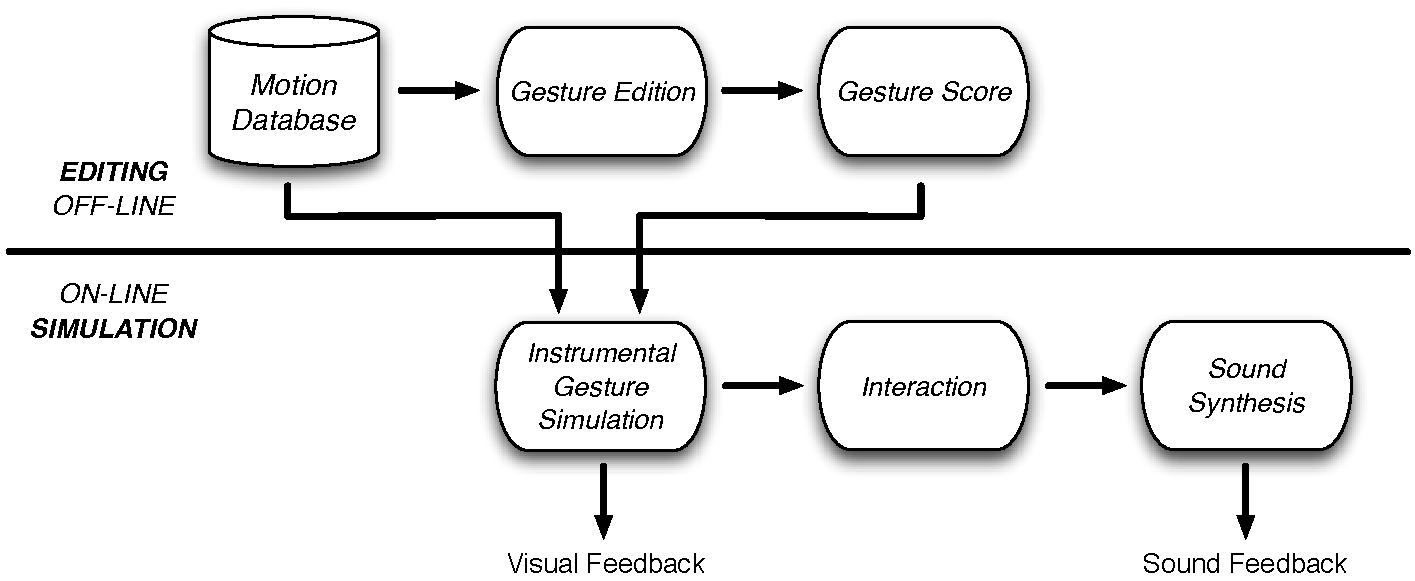
\includegraphics[width=0.9\columnwidth]{Chapters/6/Pics/Pdf/globalFramework}
	\end{center}
	\vspace{-0.5cm}
	\caption{Global approach to the composition process of virtual percussion performances.}
	\label{fig:composition}
\end{figure}

%%%%%%%%%%%%%%%%%%%%%%%%%%%%%%%%%%%%%%%%%%%%%%%%%%%%%%%%%%%%%%%%%%%%%%%%%%%%%%%%%%%%%%%%%%%%%%%%%%%%%%%%%%%%%%%%%%%%


%%%%%%%%%%%%%%%%%%%%%%%%%%%%%%%%%%%%%%%%%%%%%%%%%%%%%%%%%%%%%%%%%%%%%%%%%%%%%%%%%%%%%%%%%%%%%%%%%%%%%%%%%%%%%%%%%%%%

	\section{Gesture Edition and Composition}
	\label{sec:Music_Composition}

The synthesis system presented in the previous chapter is used for creating novel percussion sequences from available motion data. We detail in this section the motivation and mechanisms involved during the edition of gesture scores that are simulated by our synthesis system. We consider this edition step as a first advance towards the composition of virtual music performances with our system.\\

The basis of the presented edition process is highly inspired from existing works in representing music-related materials. Since the beginning of the transcription of music performances, composers and performers have used the idea of representing sounds as independent and distinct events. The most obvious example of this idea is of course the transcription of notes on music scores. This event-based representation can be more or less suited depending on the considered music performance. For example, it is useful for representing sounds produced by instruments that involve distinct actions, such as striking or plucking. For other instruments involving continuous actions, such as a vibrating reed or bowing, such representation can also be useful by defining events with a start, an end, a state change. This is namely the approach that was adopted in the design of the widespread \emph{MIDI} protocol \citeCM{midi}.

Similarly, we define a set of events that can be used in our system for synthesizing percussion performances. However, the drastic difference from the previously detailed event representation is that our system uses the manipulation of elementary \emph{gesture events}. In fact, these gesture events are consituted of motion signals coming directly from motion data presented in chapter \ref{chapter:Analysis}. We will therefore refer to them as \emph{gesture units}. \myfigname \ref{fig:composition} depicts the use of these gesture units in our synthesis system. The edition and assembling of these canonical gesture units leads to the specification of a \emph{gesture score}, whose equivalent signal is then simulated by our system.

\begin{figure}%[H]
	\begin{center}
%		\subfigure[]{\label{fig:grips1}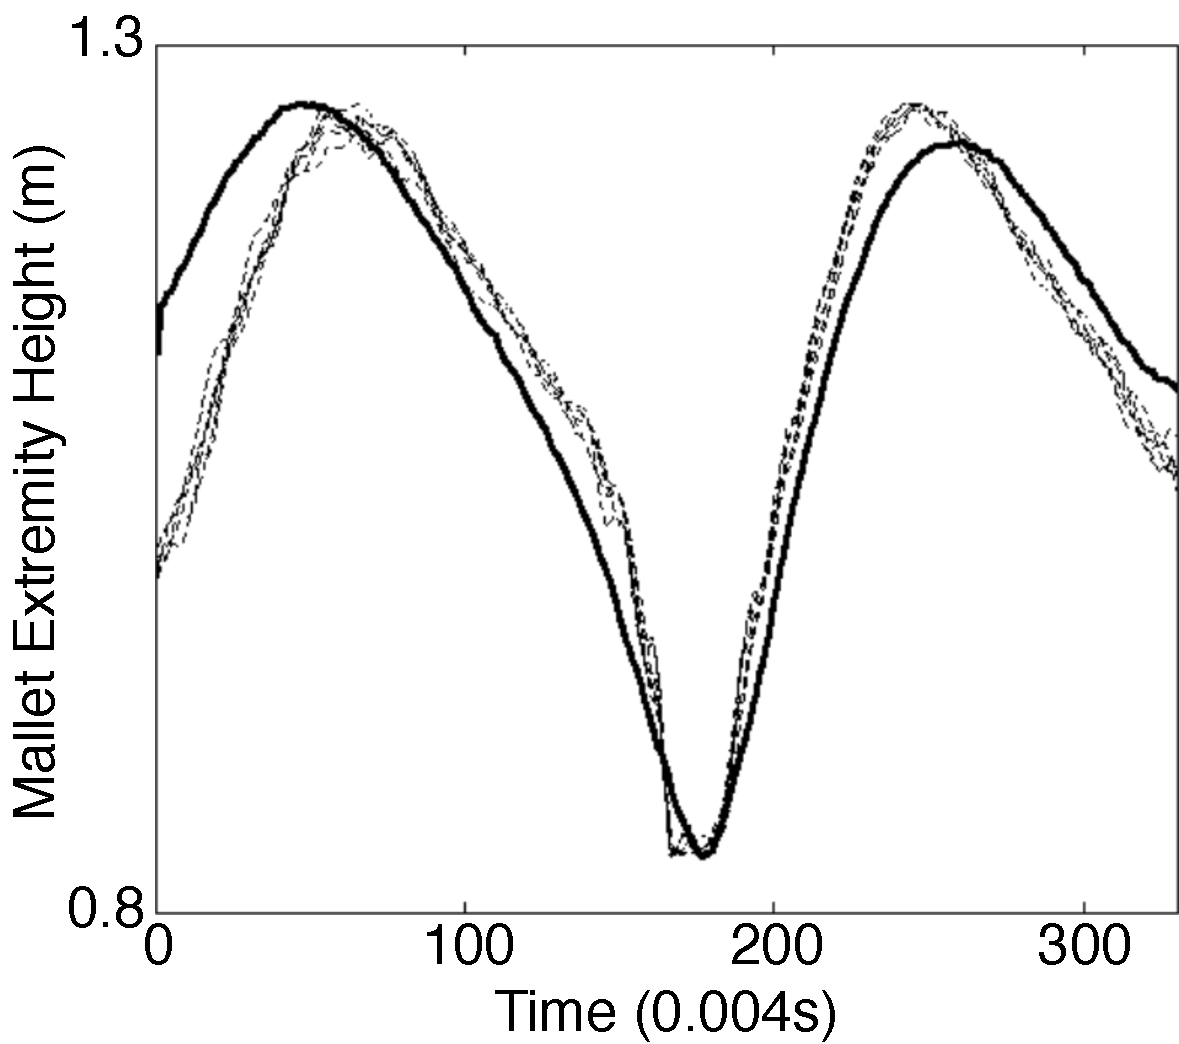
\includegraphics[width=0.325\columnwidth]{Chapters/6/Pics/Pdf/frenchGripUnitsCurves.pdf}}
%		\subfigure[]{\label{fig:grips1}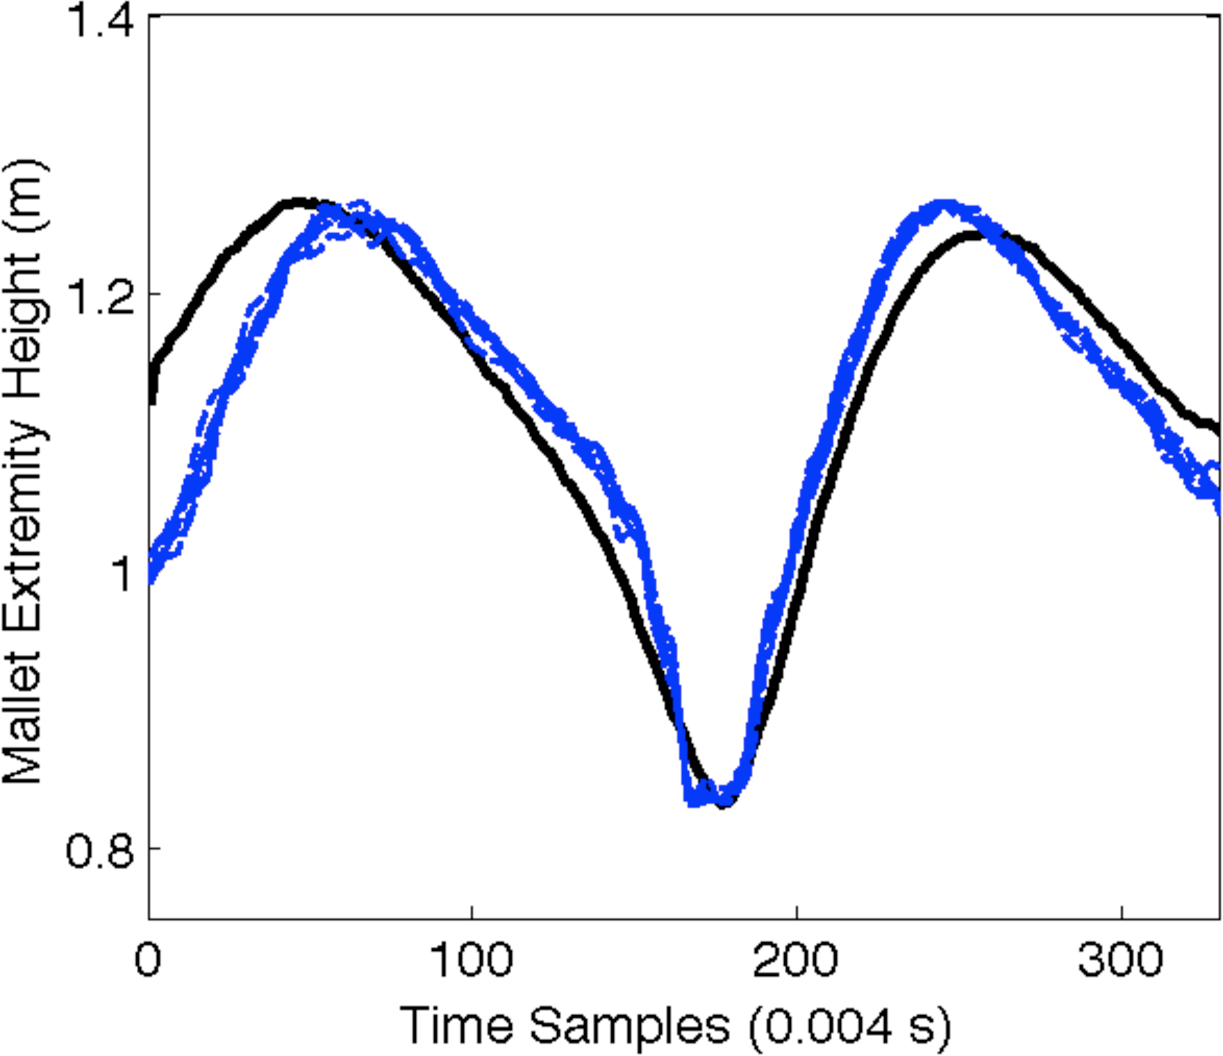
\includegraphics[width=0.45\linewidth]{Chapters/6/Pics/Pdf/frenchGripUnits2.pdf}}
		\subfigure[]{\label{fig:grips1}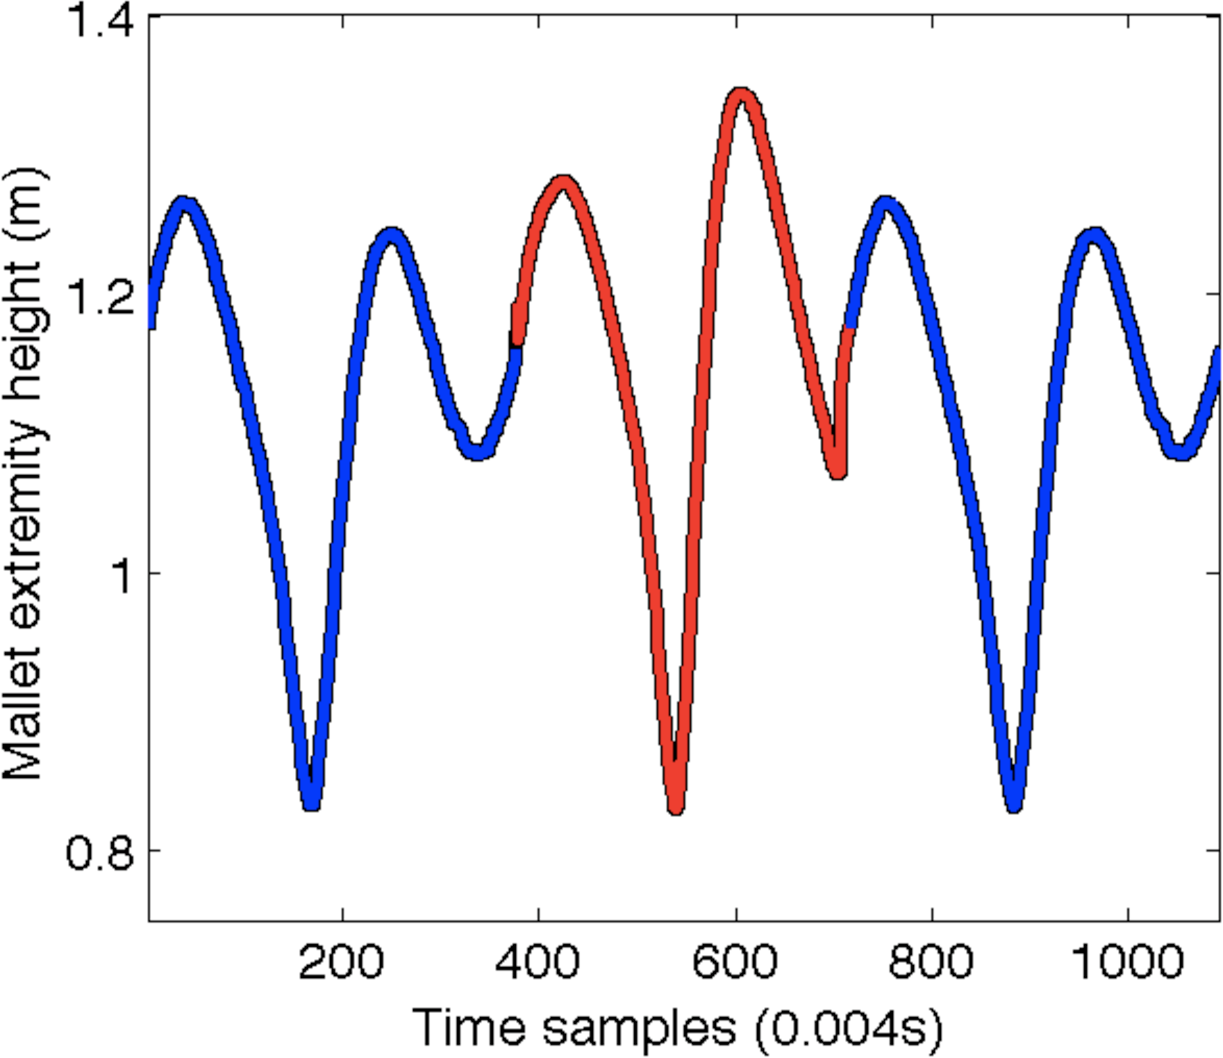
\includegraphics[width=0.45\linewidth]{Chapters/6/Pics/Pdf/articulation1.pdf}}
		\hspace{6mm}
%		\subfigure[]{\label{fig:grips2}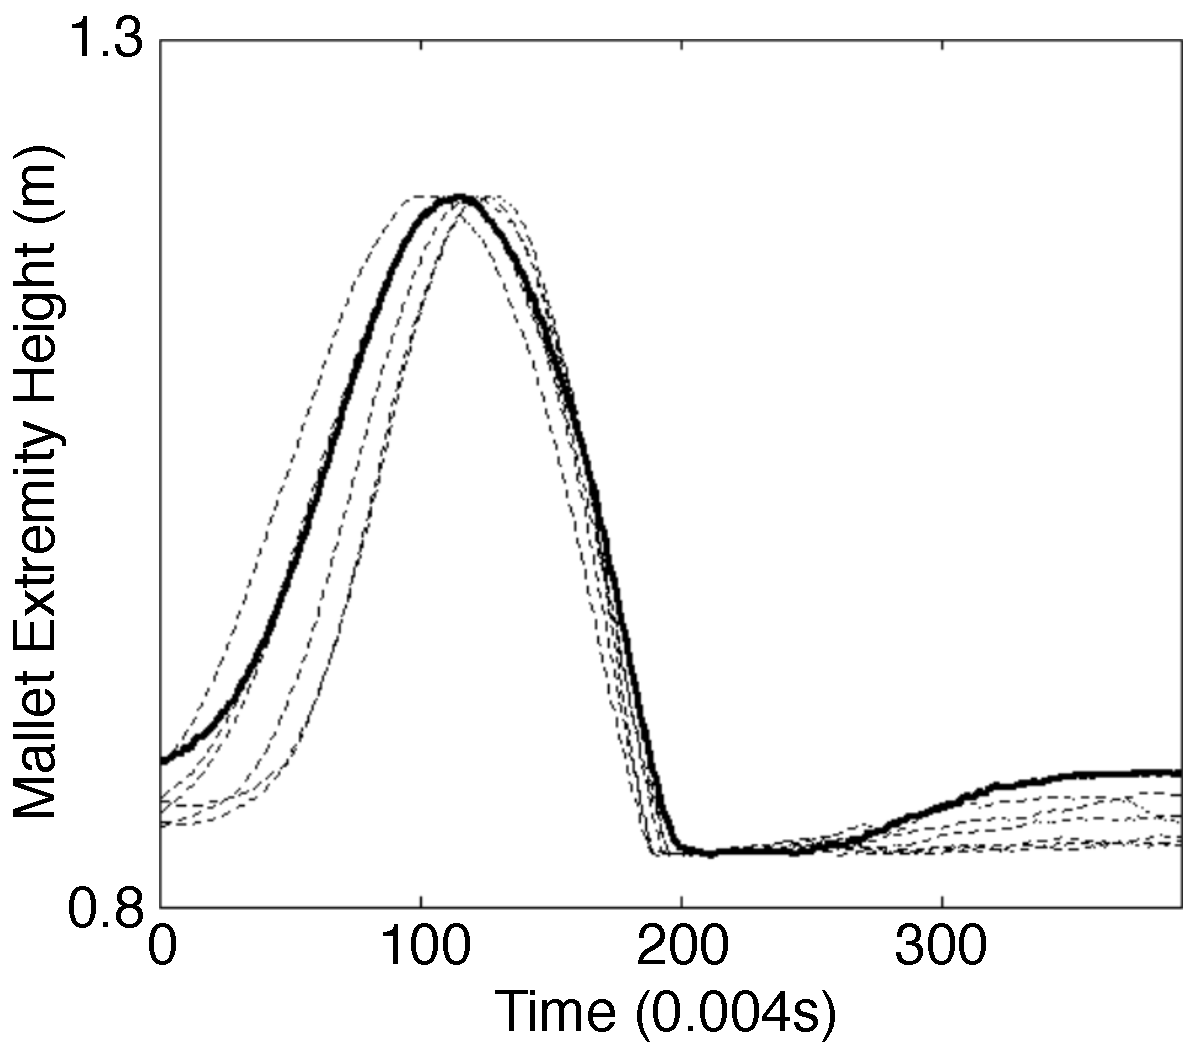
\includegraphics[width=0.325\columnwidth]{Chapters/6/Pics/Pdf/germanGripUnitsCurves.pdf}}
%		\subfigure[]{\label{fig:grips2}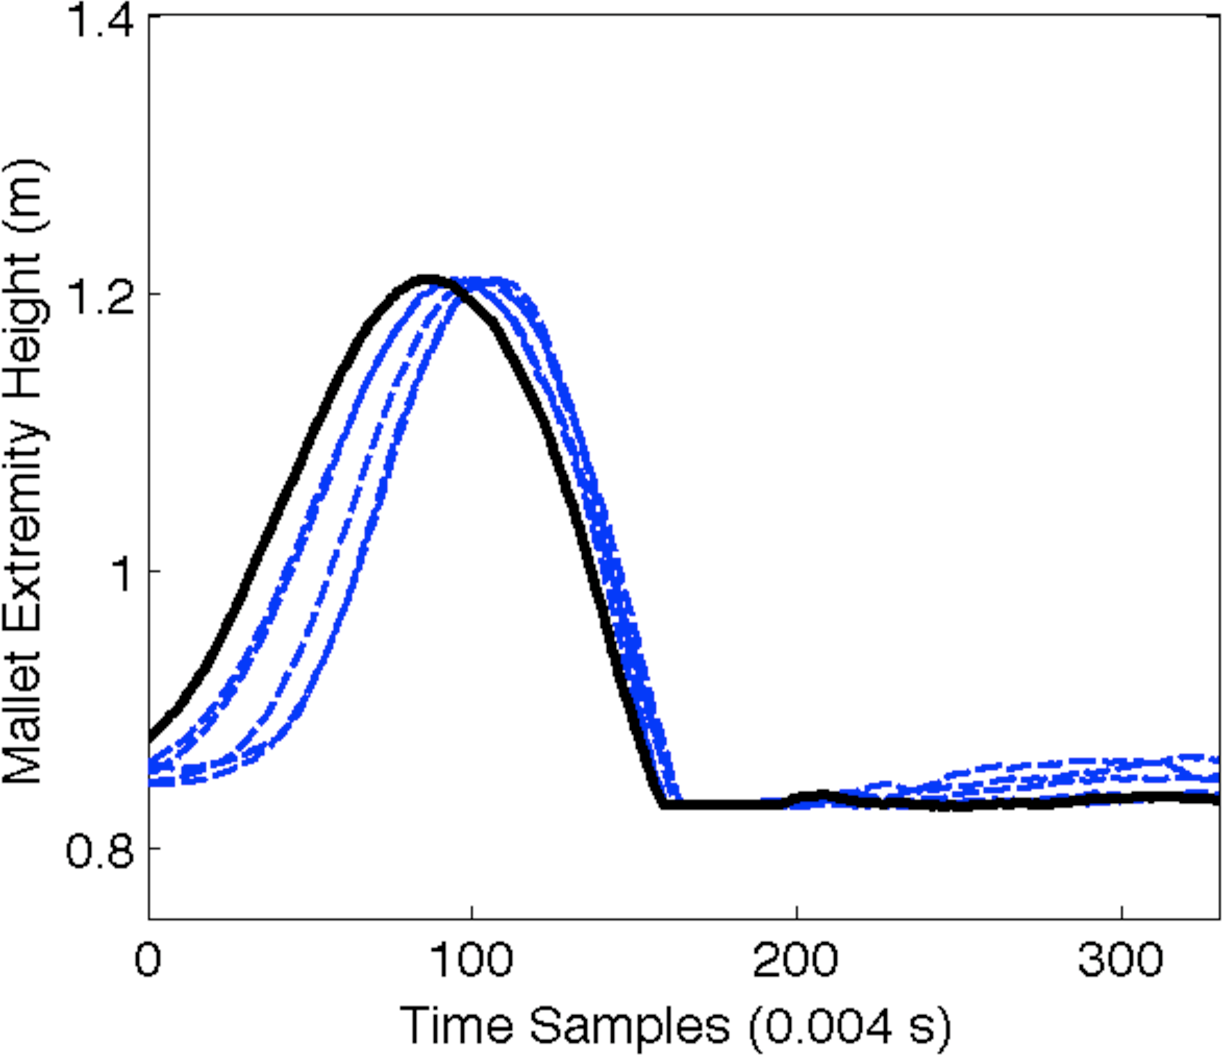
\includegraphics[width=0.45\linewidth]{Chapters/6/Pics/Pdf/germanGripUnits2.pdf}}
		\subfigure[]{\label{fig:grips1}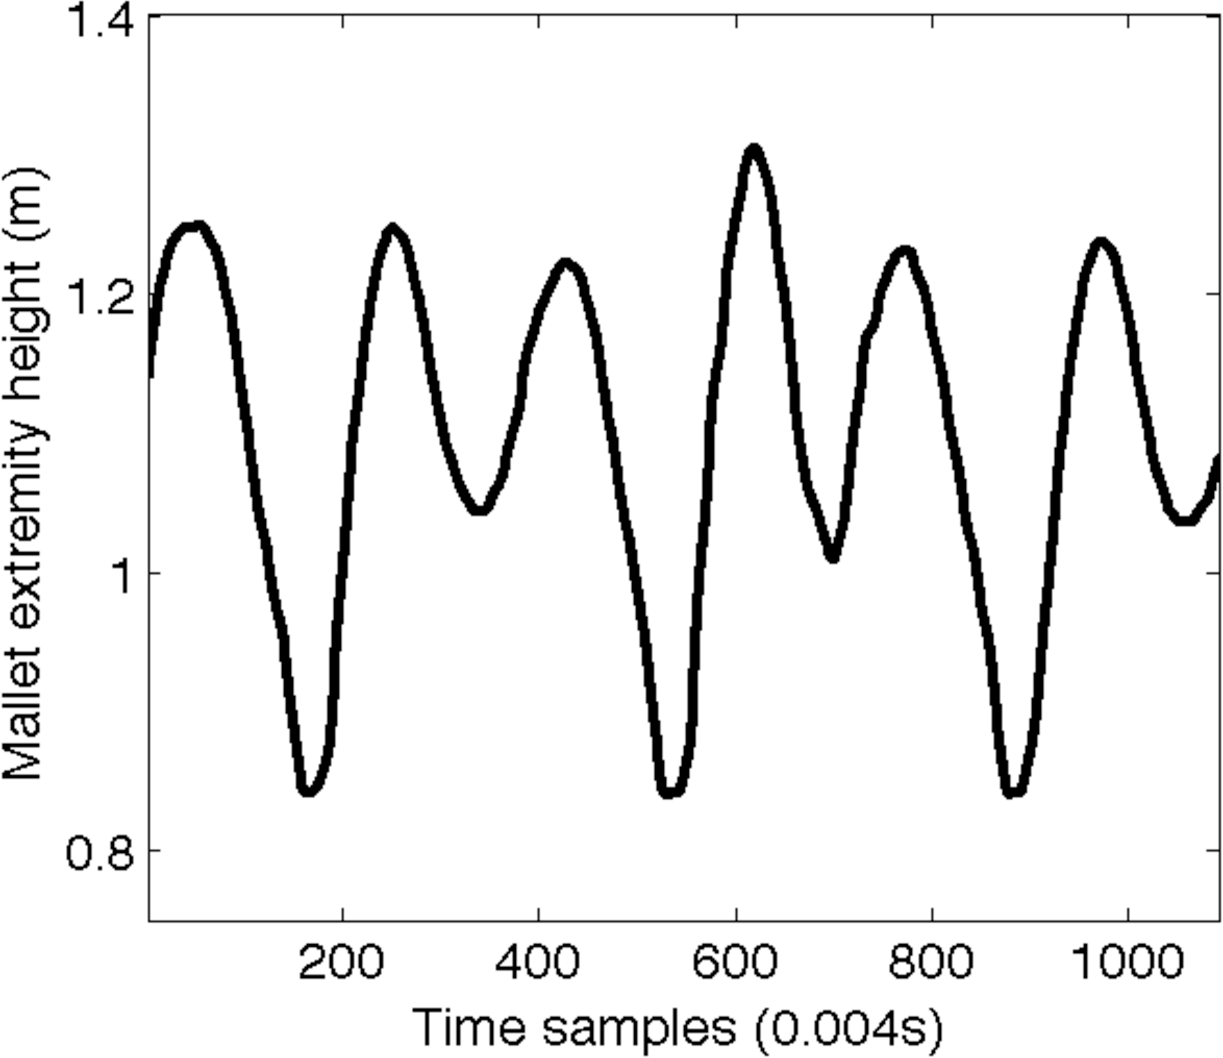
\includegraphics[width=0.45\linewidth]{Chapters/6/Pics/Pdf/articulation2.pdf}}
	\end{center}
	\vspace{-0.5cm}
	\caption[Gesture edition and composition]{Gesture edition and composition: (a) \emph{beat-centered} gesture units for \emph{legato} (blue) and \emph{accent} (red) playing modes, (b) resulting simulation of the assembling of the two units.}
	\label{fig:FrenchGermanGrips_Sim}
\end{figure}
		
Our edition and composition process of gesture scores makes available gesture units of different types. These gesture units are directly related to the motion capture database, so that a huge amount of gesture units are available for representing the playing techniques under study (grips, playing modes, beat locations). We detail here how these gesture units are obtained, as well as how gesture scores are edited from these latter. This involves both an adequate segmentation of motion capture data, as well as an assembling (composition) of the resulting gesture units.\\

An interesting technical question here is the way the simulation step uses the edited gesture scores. The segmentation process discussed in section \ref{subsec:Analysis_TimpaniAnalysis_Segmentation} leads to \emph{beat-to-beat} gesture units for each of the playing techniques under study. It should be noted however that gesture scores involving such \emph{beat-to-beat} gesture units are not usable in a simulation context. This segmentation creates two types of problem. The first one is related to the fact that linking two gesture units at the moment of the beat impact may create unwanted kinematic discontinuities, concerning the position and orientation (and their derivatives) of both mallet extremities and body segments. Another problem that can occur is the alteration of beat impact profiles. Linking two gesture units at the beat impact would lead to separate impact profiles in two phases, which may results in the modification of the action/reaction mechanical nature of the impact. Finally, placing the articulation point between two gesture units during the beat impact disagrees with the usual decomposition of instrumental gestures into preparatory, interaction and retraction gestures.

%since it would imply that the articulation point between gesture units is achieved during beat impact contacts. This segmentation choice creates issues from a simulation point of view, since the end and start of two gesture units often show differences in position and orientation of the rigid bodies composing the virtual character. Managing the transition between two gesture units this way may create unwanted motion effects since the contact of the mallet with the drum membrane create external forces that act on these rigid bodies. Such transition during the contact with the drum membrane could also have a dramatical effect on the simulated beat impact. Furthermore, such transition disagrees with the usual decomposition of instrumental gestures into preparatory, interaction and retraction gestures.

We therefore translate gesture units from \emph{beat-to-beat} to \emph{beat-centered} units. Handling the articulation between gesture units in such a way is more consistent since the articulation point is placed between the retraction phase of the previous gesture unit and the preparatory phase of the next one. However, even such a unit representation may lead to discontinuities in position and velocity between two gesture units. That is why we ensure a C$^1$ continuity on drumstick extremity trajectories. Examples of \emph{beat-centered} gesture units for \emph{legato} and \emph{accent} playing modes are presented in \myfigname \ref{fig:FrenchGermanGrips_Sim}, with the corresponding simulation of the assembling of the two units.\\

Another issue to discuss concerning the edition of gesture scores is the way the gesture units are assembled to create a partition that our system will simulate. This includes two underlying questions, on the one hand which gesture unit will be chosen for representing a playing technique since many units are available, and on the other hand how the assembling is practically achieved?

The equivalent problem to the first question brings back, for a given playing technique, to the existence of a "best-suited" gesture unit among the available ones. This issue has also been under study in \citeCM{ramstein:PhD91} concerning piano fingering. Our viewpoint on this open question is to argue that performers are highly trained to replicate and adapt their  gestures under a wide range of conditions. So that our solution is to pick up a particular gesture unit in a captured sequence, apart from the first and last one. This restriction ensures that no external disturbance is included in the gesture unit, as it was observed that performers tend to test the balance of their mallets at the beginning of a sequence, and exaggerate their motion when finishing it.

Once a set of gesture units is available for representing each playing technique, a strategy has to be developped for assembling these in a whole coherent gesture score. This includes again two underlying problems. The first one concerns the articulation between different position and orientation postures of the virtual character from the end of a gesture unit to the beginning of the next one. In all the percussion exercises presented in this chapter, this problem was achieved mainly by focusing only on the mallet extremity trajectories, as these latter are essential factors in percussion gestures as underlined in chapter \ref{chapter:Analysis}. The choice of the gesture units was therefore achieved by a careful analysis of the height of mallet extremity trajectories so that a match can be found between the end of a gesture unit and the beginning of the next one. The animation engine then involves an interpolation process for transitioning from a gesture unit to another. The second problem concerns the timing issue when mixing heterogenous gesture units. It has been easily overcome due to the high proficiency of performers in keeping a steady tempo.

%sketching, issue: position, orientation => interpolation; timing

%Another limiting issue is the choice of the gesture units used during the editing step. Such issue yields inevitably to the question of the existence of a best-suited gesture unit, compared to other examples of the same playing mode. If such "best" gesture unit exists, how can one identify it among the numerous replicates available in the motion database? Otherwise, does it make sense to average multiple gesture units so that a "mean" gesture unit can be used? We believe that using an average gesture might lead to the loss of some expressive features implicitly contained in the gesture signal. We therefore chose one specific gesture example within the sequence, without trying to find an optimized criteria for selecting this gesture unit. %[Can you comment on the consequences of this arbitrary choice?]


%%%%%%%%%%%%%%%%%%%%%%%%%%%%%%%%%%%%%%%%%%%%%%%%%%%%%%%%%%%%%%%%%%%%%%%%%%%%%%%%%%%%%%%%%%%%%%%%%%%%%%%%%%%%%%%%%%%%


%%%%%%%%%%%%%%%%%%%%%%%%%%%%%%%%%%%%%%%%%%%%%%%%%%%%%%%%%%%%%%%%%%%%%%%%%%%%%%%%%%%%%%%%%%%%%%%%%%%%%%%%%%%%%%%%%%%%

	\section{Musical Evaluation of Virtual Percussion Performances}
	\label{sec:Music_Evaluation}

One of the most interesting outcomes of such framework is the possibility of handling and assembling heterogeneous performances using a combination of a few percussion gesture units. Thanks to the physics simulation of the virtual performer, the issue of gesture articulation between movement units is partly addressed by the physics engine, thus leading to a more natural sequence of movements\footnote{The resulting articulation is not necessarily equivalent to real performer techniques. It will nevertheless be a physically plausible solution to the problem.}.\\

\begin{table}%[H]
	\centering
	\caption{Timpani playing notation}
	\begin{tabular}{||x{2.3cm}|x{2.3cm}|x{2.3cm}|x{2.3cm}|x{2.3cm}||} \hline
		\small{$Legato$} & \small{$Tenuto$} & \small{$Accent$} & \small{$V.Accent$} & \small{$Staccato$}		\tabularnewline \hline \hline
		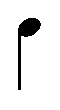
\includegraphics[height=10.8mm]{Chapters/6/Pics/Pdf/legato} & 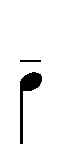
\includegraphics[height=16mm]{Chapters/6/Pics/Pdf/tenuto} & 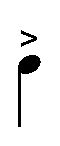
\includegraphics[height=14.1mm]{Chapters/6/Pics/Pdf/accent} & 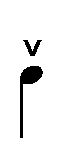
\includegraphics[height=15.2mm]{Chapters/6/Pics/Pdf/verticalaccent} & 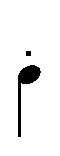
\includegraphics[height=15.5mm]{Chapters/6/Pics/Pdf/staccato} 	\tabularnewline \hline \hline
		\small{$One-Third$} & \small{$Center$} & \small{$Rim$} & \small{$Left$} & \small{$Right$}		\tabularnewline \hline \hline
		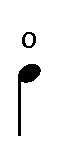
\includegraphics[height=15.5mm]{Chapters/6/Pics/Pdf/onethirdlocation} & 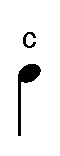
\includegraphics[height=15.5mm]{Chapters/6/Pics/Pdf/centerlocation} & 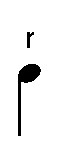
\includegraphics[height=15.5mm]{Chapters/6/Pics/Pdf/rimlocation} & 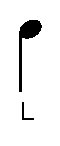
\includegraphics[height=13.8mm]{Chapters/6/Pics/Pdf/leftbeat} & 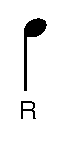
\includegraphics[height=13.8mm]{Chapters/6/Pics/Pdf/rightbeat} 	\tabularnewline \hline
	\end{tabular}
	\label{tab:notation}
\end{table}

To evaluate the proposed framework, we have simulated an extensive set of musical examples consisting of several timpani exercises\footnote{The exercises presented in this chapter are available at\\ \href{http://www-valoria.univ-ubs.fr/Alexandre.Bouenard/index.php/Research/PhDThesis}{http://www-valoria.univ-ubs.fr/Alexandre.Bouenard/index.php/Research/PhDThesis}}. The resulting simulations were evaluated by the last author (a University Percussion Professor and an active Performer)\footnote{Prof. F. Marandola (Schulich School of Music, McGill University) has chosen the percussion exercises to be simulated by the virtual character. He also qualitatively evaluated the synthesized percussion exercises.}, by focusing both on the visual and auditory feedback, first simultaneously and then separately. The exercises are divided in two main categories: validation and extrapolation exercises.\\

The first category, validation exercises, aims at verifying the accuracy with which the proposed framework can synthesize percussion movements (and sounds) similar to the captured movements in the database. They consist in independent exercises that explore variations on the type of grip (\emph{French} or \emph{German}), the type of playing mode (\emph{legato}, \emph{tenuto}, \emph{accent}, \emph{vertical accent} and \emph{staccato}), as well as the position of the impact on the drum membrane (one-third, center or rim).\\

The second category, extrapolation exercises, consist in musical excerpts that go beyond those obtained with motion capture. Such exercises were not performed by the musicians and therefore no articulation data corresponding to these exercises are available. They typically mix various types of gestures and impact positions in one excerpt, as well as variations on the tempo of the performances.\\

Throughout this section, all percussion exercises exploit gesture units in the motion capture database described in section \ref{sec:Analysis_MoCapDatabase}. The notation corresponding to timpani playing techniques is described in \mytabname \ref{tab:notation}, and is used as the standard notation throughout the rest of this paper for describing percussion exercise scores.


		\subsection{General Comments}
		\label{subsec:Music_Evaluation_GeneralCommments}

Although the simulations look and sound realistic, a first musical evaluation was achieved for determining the overall degree of expertise of the virtual performer. From the resulting simulations, we can see that the virtual timpanist's performance is similar to that of a beginner/intermediate performer.
Only part of the attacks were performed correctly, but with a wide range of variation in the impact locations and in the motion of the arm and forearm.
Other issues in the simulations include the fact that the grip is not as realistic as expected. Moreover, the bottom part of the virtual character's body does not move. This fact may be of little importance for a set of repeated notes at a steady tempo, but becomes more significant when variations in location, intensity, types of attack and rhythm occur.\\

The setup described in section \ref{sec:Analysis_MoCapDatabase} actually does not include the recording of the subtleties occurring in the mallet grips, since no sensors are monitoring the grasp mechanisms involving the fingers and the mallets. Although our motion capture setup does capture the orientation of hands and mallets, this information is not sufficient for modeling the grasp subtleties that could enhance the realism of the resulting grip simulations. Furthermore, no balance strategies are involved in the simulation of the percussion exercises, although information on performers' center of mass was captured in the motion capture sessions. This simulation choice explains the remark on the quite static bottom part of the virtual performer.


		\subsection{Validation Exercises}
		\label{subsec:Music_Evaluation_Validation}

In this section we analyze how the system manages to connect independent gesture units taken from the timpani database, where each exercise consists in a sequence of similar types of strokes. The strokes are chosen from pre-selected gesture units, corresponding to a given grip, a playing mode and a location on the timpani.
We focus on the qualitative evaluation of the simulation of playing modes as well as beat impact locations\footnote{The simulation quality of \emph{French} or \emph{German} grips is further discussed in section \ref{subsubsec:AL_IGS_L}. }.

We simulated five exercises consisting of 13 strokes each (7 for the right hand and 6 for the left hand) for each playing mode. \myfigname \ref{fig:validation1} shows an example of an exercise consisting only of \emph{legato} strokes, whereas \myfigname \ref{fig:validation2} shows the simulation score of beat impacts locations at the rim of the timpani membrane.\\

\begin{figure}%[H]
	\begin{center}
		\subfigure[]{\label{fig:validation1}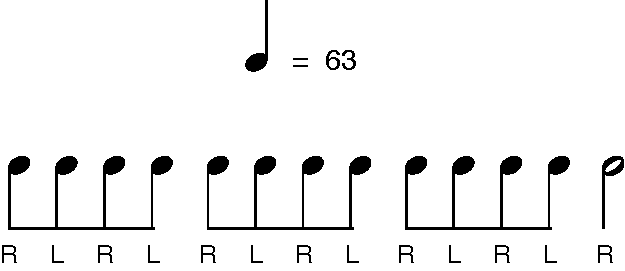
\includegraphics[width=52mm]{Chapters/6/Pics/Pdf/exo1-1.pdf}}
		\hspace{1cm}
		\subfigure[]{\label{fig:validation2}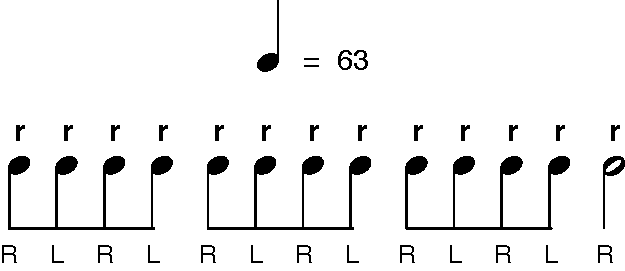
\includegraphics[width=52mm]{Chapters/6/Pics/Pdf/exo5-3.pdf}}
	\end{center}
	\vspace{-0.5cm}
	\caption[Simulated exercises: validation of playing modes and impact locations]{(a) Simulation exercise consisting of a sequence of \emph{legato} strokes. (b) Simulation exercise consisting of a sequence of \emph{legato} strokes played at the rim.}
	\label{fig:gesture}
\end{figure}

As expected, the resulting simulations show significant variations in the quality of the attacks for a given type of stroke, specifically with respect to the location of the impact point. However, the shoulders present very large movements; there is an excessive shoulder rotation for each single stroke, making the position of the elbows not accurate. In fact, given the steady position of the bottom part of the body, there should be more motion at the elbows.

The exaggeration in shoulder and elbow movements can be attributed to the physical model of the virtual percussionist. Just as any physical entity, the body parts of the virtual percussionist are characterized by inertia properties. When the physical model is put into motion, these body parts seem to acquire too much inertia, so that even if the overall motion (mallet extremities) is accurate enough compared to the recorded gesture units \cite{bouenard:AAA09}, an exaggeration of motion appears.\\

Considering only the sound generated, one can notice that the sound outcome is plausible and that playing modes producing them are audibly perceptible. However, the sound starts with too much attack (there is even some saturation at the beginning of the sound) and the resonance differs from a real timpani sound. Finally, the sound is not metallic enough when considering the attacks near the rim of the membrane.

These issues concern the \emph{Modalys} model of the drum membrane. The lack of sound resonance is easily explained by the fact that the drum membrane model does not feature a resonance body. Moreover, the non-metallic nature of the resulting sounds may also come from a combination of imprecisions both from the drum membrane model itself since no metallic rim is included in the \emph{Modalys} model, and from beat impact locations inaccuracies.


		\subsection{Extrapolation Exercises}
		\label{subsec:Music_Evaluation_Extrapolation}

The previous exercises consisted of simple sequences of similar strokes. Much more interesting though is to verify how the framework can deal with gestures combinations of different stroke types, tempos, and impact locations that were not initially recorded in sequence. Various combinations of gestures will be analyzed in the following subsections.


			\subsubsection{Playing Modes}
			\label{subsubsec:Music_Evaluation_Extrapolation_GestureVariations}
		
The following two exercises show a combination of gesture units for various playing modes. The idea is to show that the system can connect independent gesture units of each playing mode, as well as creating the articulation for a combination of these different units.

\begin{figure}%[H]
	\begin{center}
		\subfigure[]{\label{fig:gesture1}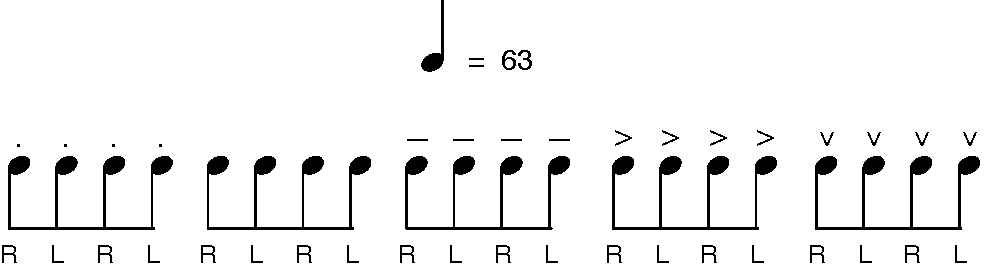
\includegraphics[width=82mm]{Chapters/6/Pics/Pdf/exo2-1.pdf}}
		\hspace{0.5cm}
		\subfigure[]{\label{fig:gesture2}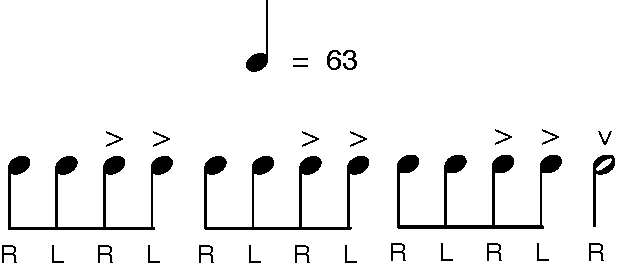
\includegraphics[width=51mm]{Chapters/6/Pics/Pdf/exo4-5.pdf}}
	\end{center}
	\vspace{-0.5cm}
	\caption[Simulated exercises: extrapolation of playing modes]{(a) Simulation exercise consisting of five gesture units repeated four times: \emph{staccato}, \emph{legato}, \emph{tenuto}, \emph{accent} and \emph{vertical accent}, respectively. (b) Simulation exercise consisting of variations between \emph{legato} and \emph{accent} strokes, ending with a \emph{vertical accent}.}
	\label{fig:gesture}
\end{figure}

The first exercise (\myfigname \ref{fig:gesture1}) is a sequence of several strokes (respectively \emph{staccato}, \emph{legato}, \emph{tenuto}\emph{accent} and \emph{vertical accent}) in groups of four strokes (two per arm). The second exercise (\myfigname \ref{fig:gesture2}) changes the type of stroke for each arm from \emph{legato} to \emph{accent} and back, finishing with a \emph{vertical accent} performed with the right hand.\\
		
Considering the articulation between the simulated playing modes, it can be seen that articulation changes are perceptible throughout the simulation. However, problems arise in \emph{legato}-\emph{tenuto} and \emph{tenuto}-\emph{accent} pairs, so that differences between these are sometimes not very clear. These can be the result of the motion exageration discussed previously (cf. section \ref{subsec:Music_Evaluation_Validation}), as well as from the fact that the effect of fingers is not available in the recorded motion data (cf. section \ref{subsec:Music_Evaluation_GeneralCommments}).

%[This may be a bit too detailed for the CMJ paper]

%For the first pair of strokes, the over motion of the shoulder in the \emph{legato} stroke masks partially the difference with the \emph{tenuto} strokes. For the second pair (\emph{tenuto-accent}), the phenomenon occurring around the fulcrum (between the thumb and the index), characterized by a change of pressure, is not perceptible, it is indeed of utmost importance to help to bring out the sharpness of the attack. 

%Again, the interpretation of the phenomena pointed out by the percussion professor comes, on the one hand, from the motion exaggeration discussed previously (cf. section \ref{subsec:validation}), and on the other hand from the fact that the effect of fingers is not available in the recorded motion data (cf. section \ref{subsec:general_commments}).\\

%As for the recognition of gesture variations from the simulated sounds, it was noted that although variation in the impact location is important throughout the exercise between \emph{legato} and \emph{accent} strokes, this variation was limited here: %[Is this right???] 
%all the \emph{legato} strokes are performed closer to the center, what helps to bring out a difference in the timbre (attack and resonance). However, these variations are too important to be able to distinguish only by listening the exact alternation of \emph{legato} and \emph{accent} strokes. % [Is there variation in the simulation or not? I am lost here!]

The resulting sounds from the articulation between various playing modes were perceptible, except for the \emph{legato}-\emph{accent} sequences. This lack may result from both the \emph{Modalys} model of the drum membrane and from the simulated articulation problem in this case as pointed out previously.


			\subsubsection{Tempo Variations}
			\label{subsubsec:Music_Evaluation_Extrapolation_TempoVariations}

We have tested the simulation of articulating the same percussion gesture (\emph{legato}) under an accelerando-decelerando musical variation\footnote{This tempo variation has not been recorded initially.}. \myfigname \ref{fig:tempo1} shows the percussion exercise simulated by the virtual percussionist. 

\begin{figure}%[H]
	\begin{center}
		\subfigure[]{\label{fig:tempo1}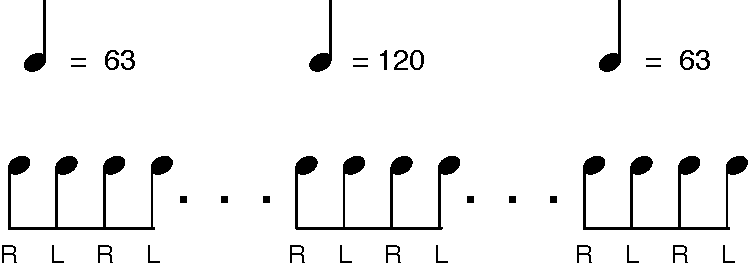
\includegraphics[width=60mm]{Chapters/6/Pics/Pdf/exo3-1.pdf}}\\
%		\hspace{1cm}
		\subfigure[]{\label{fig:tempo2}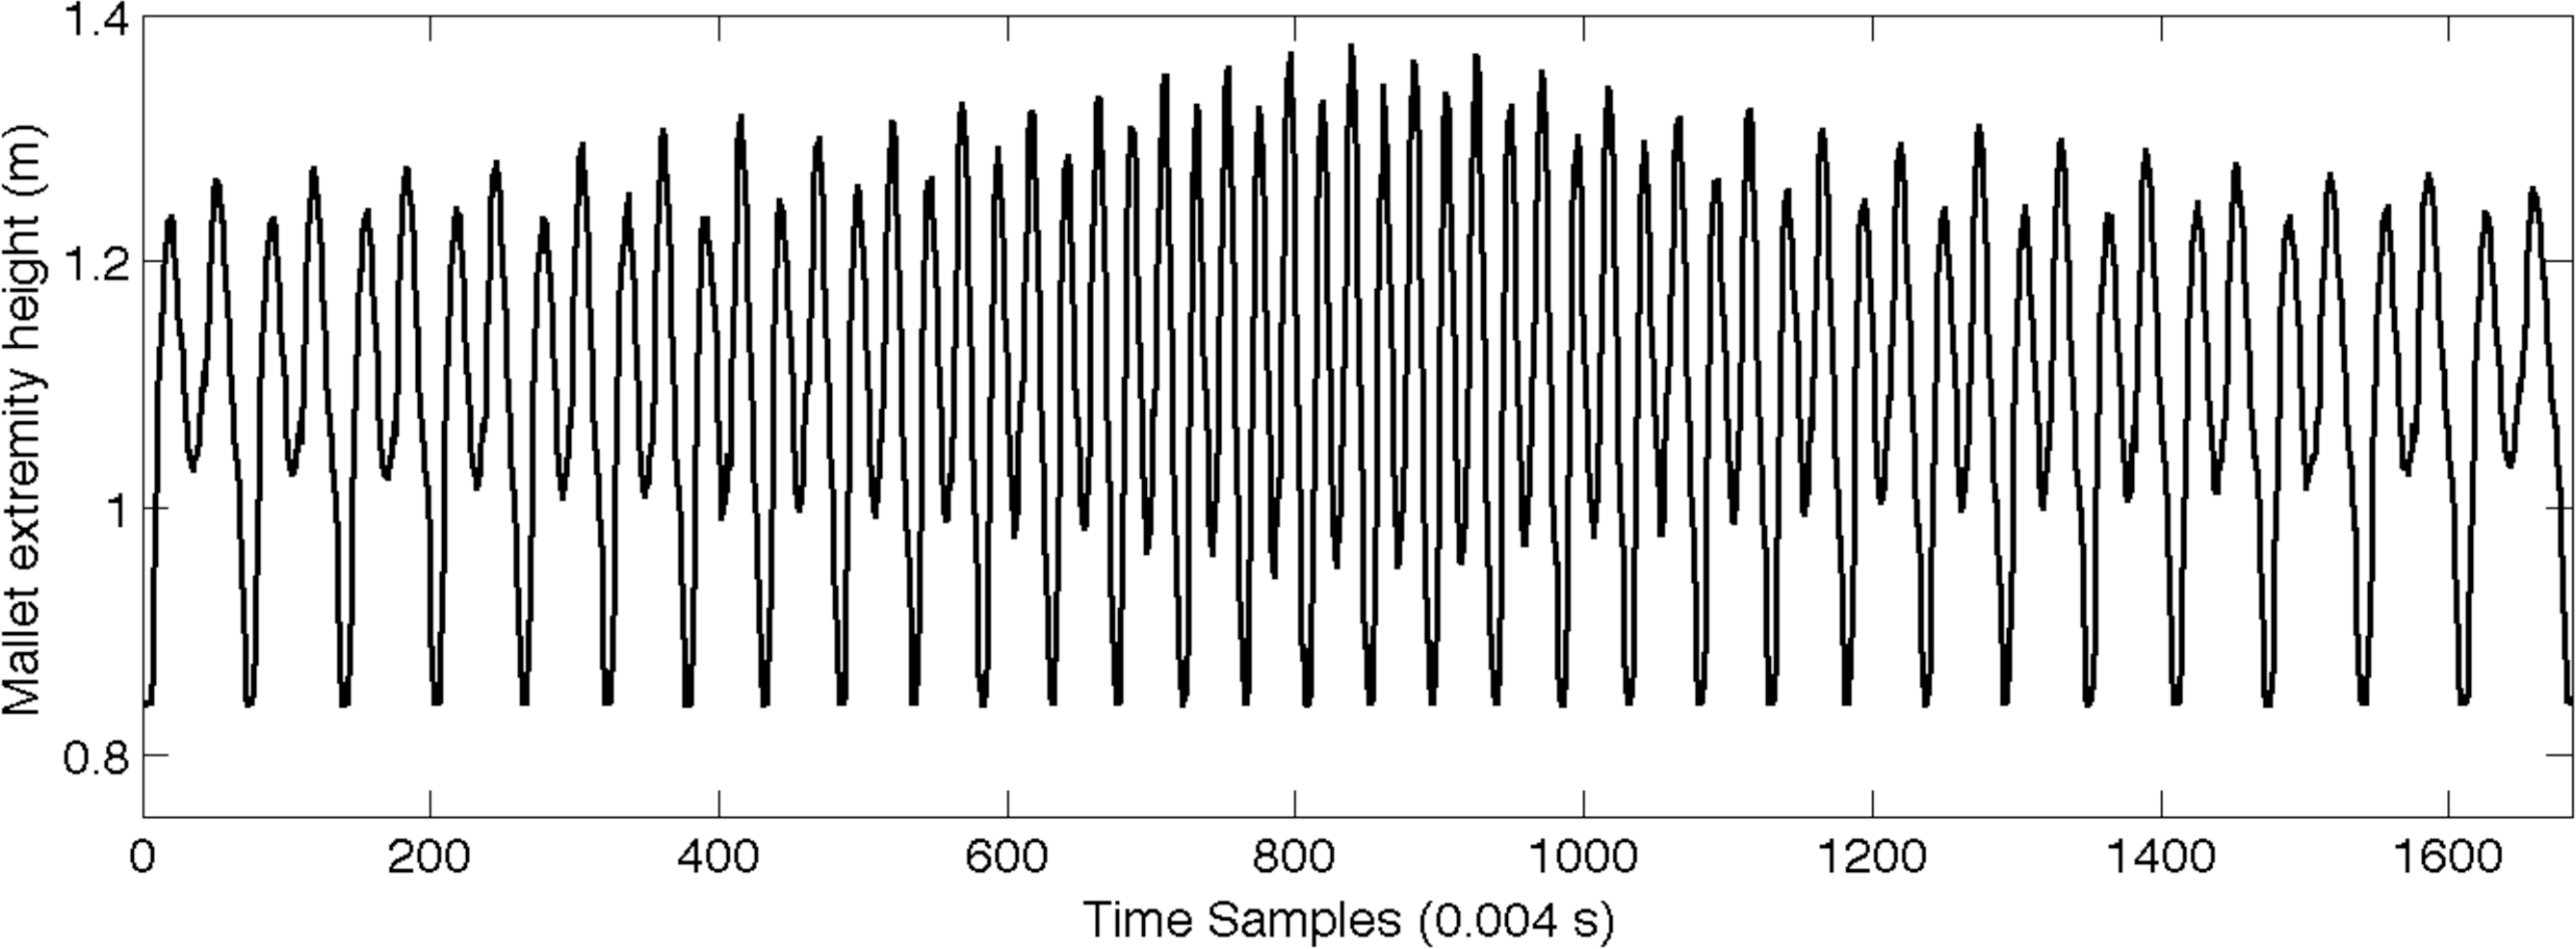
\includegraphics[width=\linewidth]{Chapters/6/Pics/Pdf/accelerandoDecelerando4.pdf}}
	\end{center}
	\vspace{-0.5cm}
	\caption[Simulated exercises: extrapolation of tempo variations]{(a) Simulation exercise consisting of an accelerando followed by a decelerando of \emph{legato} strokes. Note that the timpani mocap database only has samples of \emph{legato} strokes capture at one given tempo. (b) Simulation and articulation between \emph{legato} beats under an accelerando-decelerando musical variation (height of the tip of the mallet). %The top arrow shows an amplitude increase occurring during the accelerando, as well as small amplitude drop when approaching the maximum accelerando velocity.
}
	\label{fig:tempo}
\end{figure}

Regarding the quality of the synthesized \emph{legato} strokes under such tempo variation, it can be seen in the simulation that the motion of the shoulders increase with the speed (becoming way too wide), while the amplitude of the motion of the forearms and the space between them remain identical. In reality, timpanists would have a tendency to bring closer their forearms and to reduce the amplitude of the vertical movements of the forearms and mallets, compensating by increasing the motion of the wrists and an increased use of the fingers. Moreover, during this accelerando phase, the flow becomes more irregular and the impact locations substantially change, causing inconsistency in the quality of the sounds produced. 

%Once again, this result would be consistent with that of a beginner who would partially lose control of his motion with the increases in performance speed.
%[Maybe keep this for the conclusions?]

\myfigname \ref{fig:tempo2} displays the motion amplitude increase (mallet extremity) along the accelerando-decelerando exercise shown in \myfigname \ref{fig:tempo1}. This increase can be explained by a gain of inertia in the physical model of the virtual percussionist (cf. section \ref{subsec:Music_Evaluation_Validation}). %More interestingly, there is also an amplitude drop in the vertical motion of the mallet extremity when approaching the maximum velocity of the accelerando (see the arrow in \myfigname \ref{fig:tempo2}). This phenomenon does agree with the expected amplitude decrease expected in real performances. However, this natural amplitude drop combined with an unwanted increase of motion does not seem to be visually and auditory perceptible.

The inconsistency reported on beat impact locations can be explained from a simulation point of view. As mentioned in section \ref{subsec:Synthesis_Physics_MotionControl_CartesianSpaceControl} and emphasized by equation \ref{eq:equation3}, the control of the virtual percussionist is achieved by the control of errors between target and state mallet extremities. The accelerando phase seems to have a critical effect on the control of such errors, leading to the propagation of joint errors on the mallet extremity and on beat impact locations.\\

As for the quality of the corresponding synthesized sounds to this percussion exercise, during the accelerando, a crescendo occurs naturally by setting on resonance the membrane of timpani. It should be noticed that this feature is also used by real timpanists to build-up a crescendo during a roll: they increase the speed of their rolls to build up the crescendo while they tend to find the speed which brings out the maximum natural resonance from the timpani.

This fact attests to the natural response of the \emph{Modalys} model of the drum membrane in response to the simulated \emph{legato} strokes under an accelerando tempo variation. It shows moreover that the interaction model, and especially the collision detection of beat impacts, offers realistic features such as contact durations and forces in comparison to real timpani performances.


			\subsubsection{Impact Location Variations}
			\label{subsubsec:Music_Evaluation_Extrapolation_ImpactVariations}

\begin{figure}%[hd]
	\begin{center}
		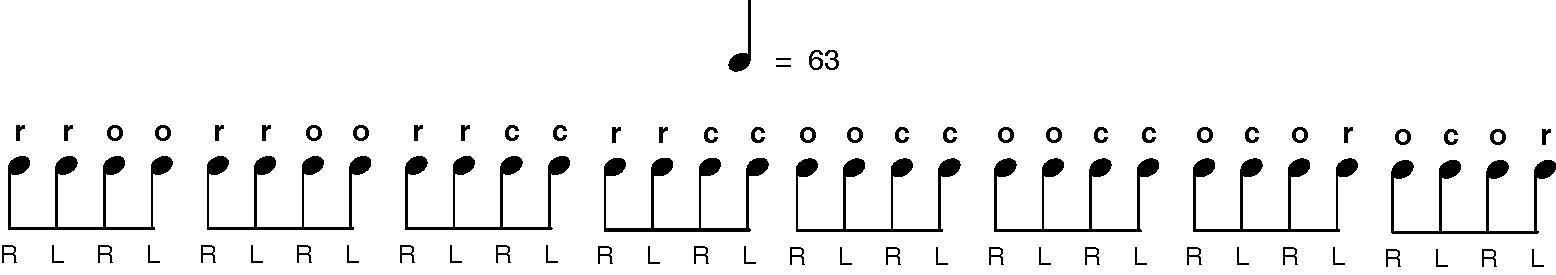
\includegraphics[width=130mm]{Chapters/6/Pics/Pdf/exo7-1.pdf}
	\end{center}
	\vspace{-0.5cm}
	\caption[Simulated exercises: extrapolation of impact location variations]{Simulation exercise consisting of several \emph{legato} strokes played at various locations in the membrane (o: one-third, c: center and r: rim).}
	\label{fig:exo7-1}
\end{figure}

Finally, we simulated the exercise depicted in \myfigname \ref{fig:exo7-1}, consisting in a sequence of several \emph{legato} strokes played at various beat impact locations. This exercise aims to verify if the articulation of various beat impact locations results in still perceptible changes in the simulation.

In fact, the differences remain perceptible, more specifically with respect to the end of the exercise (two last groups of four strokes: o c o r). However, one would expect that the differences would be more obvious among the three types of location, specifically for the centered strokes. 

The reason for this effect is that the original recorded performances that were used to build and simulate this exercise were not performed accurately enough with respect to impact position. As shown in \myfigname \ref{fig:variability}, the recorded beat impact locations (hollow signs) for the center location are too near to those corresponding to the one-third location.

%The comments underline the articulation quality between the selected gesture units for simulating different beat impact locations, and especially for the difficult task of simulating one-third, center and rim beat impact locations in a short time lapse ("o c o r"). Moreover, the percussion professor hypothesizes that the difficulty in discriminating center locations can be due to the captured gesture units used for the composition and simulation of the exercise. This hypothesis do agree with the observation of beat impact locations initially recorded. 

%%%%%%%%%%%%%%%%%%%%%%%%%%%%%%%%%%%%%%%%%%%%%%%%%%%%%%%%%%%%%%%%%%%%%%%%%%%%%%%%%%%%%%%%%%%%%%%%%%%%%%%%%%%%%%%%%%%%


%%%%%%%%%%%%%%%%%%%%%%%%%%%%%%%%%%%%%%%%%%%%%%%%%%%%%%%%%%%%%%%%%%%%%%%%%%%%%%%%%%%%%%%%%%%%%%%%%%%%%%%%%%%%%%%%%%%%
		
	\section{Discussion: Advantages and Limitations}
	\label{sec:Music_AL}

Simulating instrumental percussion gestures for controlling sound synthesis processes presents advantages and limitations, and these are of different orders when considering each module of our framework. In the following sections we will analyze in detail some of the sources of variability that are produced by our simulation system and may be at the origin of unwanted artifacts, as well as new interesting possibilities. We therefore consider sequentially the advantages and limitations of each module of our framework, considering first the instrumental gesture simulation and then the gesture edition step (cf. \myfigname \ref{fig:composition}).


		\subsection{Instrumental Gesture Simulation}
		\label{subsec:Music_AL_IGS}

We here underline the importance of the parameterization of the virtual character during the simulation. A non-optimal parameterization can lead to artifacts in the resulting synthesis of percussion performances, as well as to effects on synthesized sounds. We also highlight the interest of simulating instrumental gestures with respect to the possible modulation of synthesized gestures while preserving the initial style and expressive characteristics of real percussion performances.


			\subsubsection{Advantages}
			\label{subsubsec:AL_IGS_A}

From a simulation point of view, once an acceptable parameterization of the simulation is achieved, associating a motion capture database and the physics-based synthesis of instrumental gestures yields an accurate simulation of movements.

\begin{figure}%[H]
	\begin{center}
		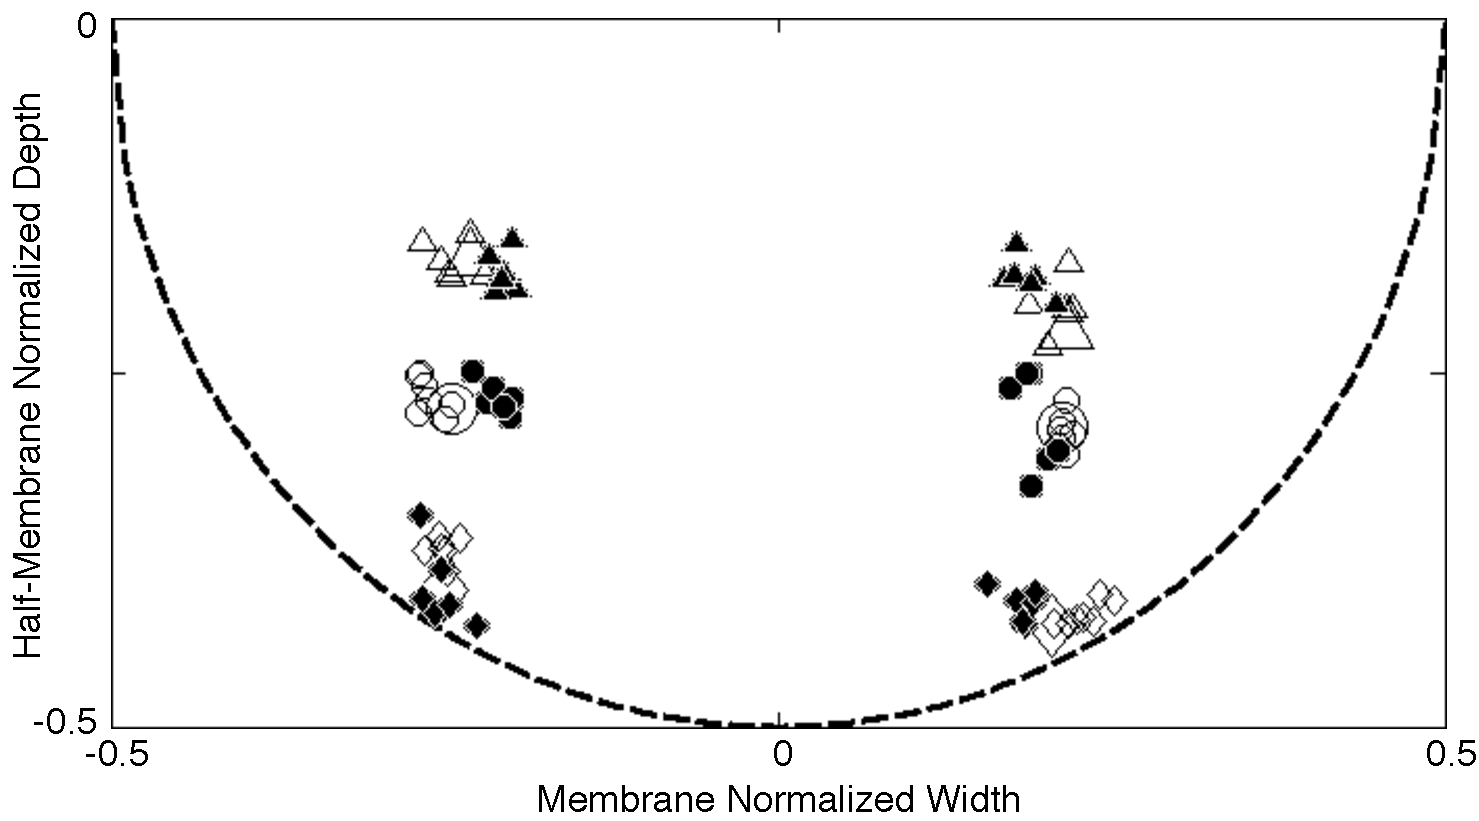
\includegraphics[width=0.8\columnwidth]{Chapters/6/Pics/Pdf/beatImpactsAnalysis2.pdf}
	\end{center}
	\vspace{-0.5cm}
	\caption[Comparison of captured and simulated beat impact locations played \emph{legato}]{Comparison of captured and simulated beat impact locations played \emph{legato}. Small hollow signs represent strokes from motion capture data, whereas large hollow signs represent beat impact locations resulting from the chosen gesture units. Bold signs represent the simulated beat impact locations.}
	\label{fig:variability}
\end{figure}
	
A first advantage of the our physics-based framework for simulating percussion gestures is the retrieval of the dynamical aspects (beat impacts) of the recorded instrumental gestures, since no extra sensors have been used during the recording of percussion performances and no information concerning beat impact durations and forces has been recorded. Such physical approach is also of great interest for exploring the interaction of percussion gestures with sound synthesis since it makes available useful contact information that can be exploited by sound synthesis processes.

A second advantage of our system is its virtual nature. Indeed, the proposed framework allows the modeling of realistic phenomena occurring during real percussion performances. Furthermore, it also allows to go beyond reality, and provides the possibility of modifying the parameters of the virtual environment as wanted for creating new percussion performances. Among these parameters, it includes modifications of the physical model of the virtual percussionist, leading for instance to various stiffness properties of the synthesized gestures. Different interaction schemes between synthesized gestures and sound synthesis inputs can also be explored.\\

From a more musical point of view, an issue to take into account is the small variations in movements that are important to produce expressive performances. Indeed, deadpan performances where movements are kept as close to an ideal movement target as possible are considered mechanical and non expressive. By choosing a single gesture unit for representing each playing mode in the various simulations, we might actually expect to eliminate the natural variability of movements from the original performance by the (real) percussionists. This choice, although greatly simplifying the simulation, has the downside of potentially creating mechanical performances.

Nevertheless, thanks to the physics simulation layer, departing from a single gesture unit for each gesture type will nevertheless produce synthesized gestures with inherent variability due to the dynamic characteristic of the virtual character. This micro variability can be explained by a combination of effects occurring at each level of our framework. As explained below, for the instrumental gesture simulation, numerical drifts can occur but still be controlled. Exploiting such drifts for slightly modifying the instrumental gesture may produce some form of expressiveness. For instance, single simulations of the same gesture unit yield slightly different yet consistent synthesized gesture units, as shown in \myfigname \ref{fig:FrenchGermanGrips_Sim}. The propagation (and not the amplification) of such numerical drifts is also influenced by the edition and the articulation of gesture units, thus leading to another source of variability during the simulation of a sequence of several gesture units. These small differences in gestural trajectories therefore lead to variations in the impact locations on the membrane, thus producing variations in corresponding synthesized sound. These different effects may be explored musically, and actually lead to non-mechanical performances by the virtual percussionist.

An example is presented in \myfigname \ref{fig:variability}, showing the simulation of several \emph{legato} strokes for the \emph{French} grip. Small hollow signs represent the 2D positions of motion captured strokes on the drum membrane respectively for the three impact positions. The three large hollow signs indicate the impact positions of the three captured strokes chosen as gesture units for each hand. Finally, the bold signs represent the various simulated strokes. One can note the comparable variability of the (real) percussionist's strokes from motion capture (small hollow signs), and the resulting variability of the synthesized strokes (small bold signs) from multiple simulations of each gesture unit.


			\subsubsection{Limitations}
			\label{subsubsec:AL_IGS_L}

Depending on the sequence and speed of the selected gestures, as well as to the fine tuning of the mechanical joints (equation \ref{eq:equation3}), simulation artifacts can appear and result in large variations in beat impact positions and forces. These variations are due to the adaptation of the physics simulation to the constraints in the movement data, and may yield unexpected sound phenomena.\\

An example is presented in \myfigname \ref{fig:soundComparison}, where the virtual musician performs a sequence of four beats played \emph{legato} with different sets of physical constraints (mechanical joints). In \myfigname \ref{fig:soundComparison1}, a simulation artifact can be observed on the third beat, that results in a larger sound waveform amplitude and sound intensity, actually masking the last beat. This artifact is removed by changing the physics constraints expressed by the damping and stiffness coefficients involved in equation \ref{eq:equation3}, as shown in \myfigname \ref{fig:soundComparison2}. In this latter case, one can see that the four beats are performed similarly, both in terms of amplitude and intensity\footnote{Sounds in both simulations have been obtained using \emph{Modalys}.}.

The parameterization of the mass and density of the different segments composing the physical model of the virtual percussionist should be chosen carefully, so that the inertial behavior of the system is comparable to that of humans. Otherwise accelerations or slowdowns as well as unexpected overruns may be obtained, leading to unrealistic simulations.

\begin{figure}[H]
	\begin{center}
		\subfigure[]{\label{fig:soundComparison1}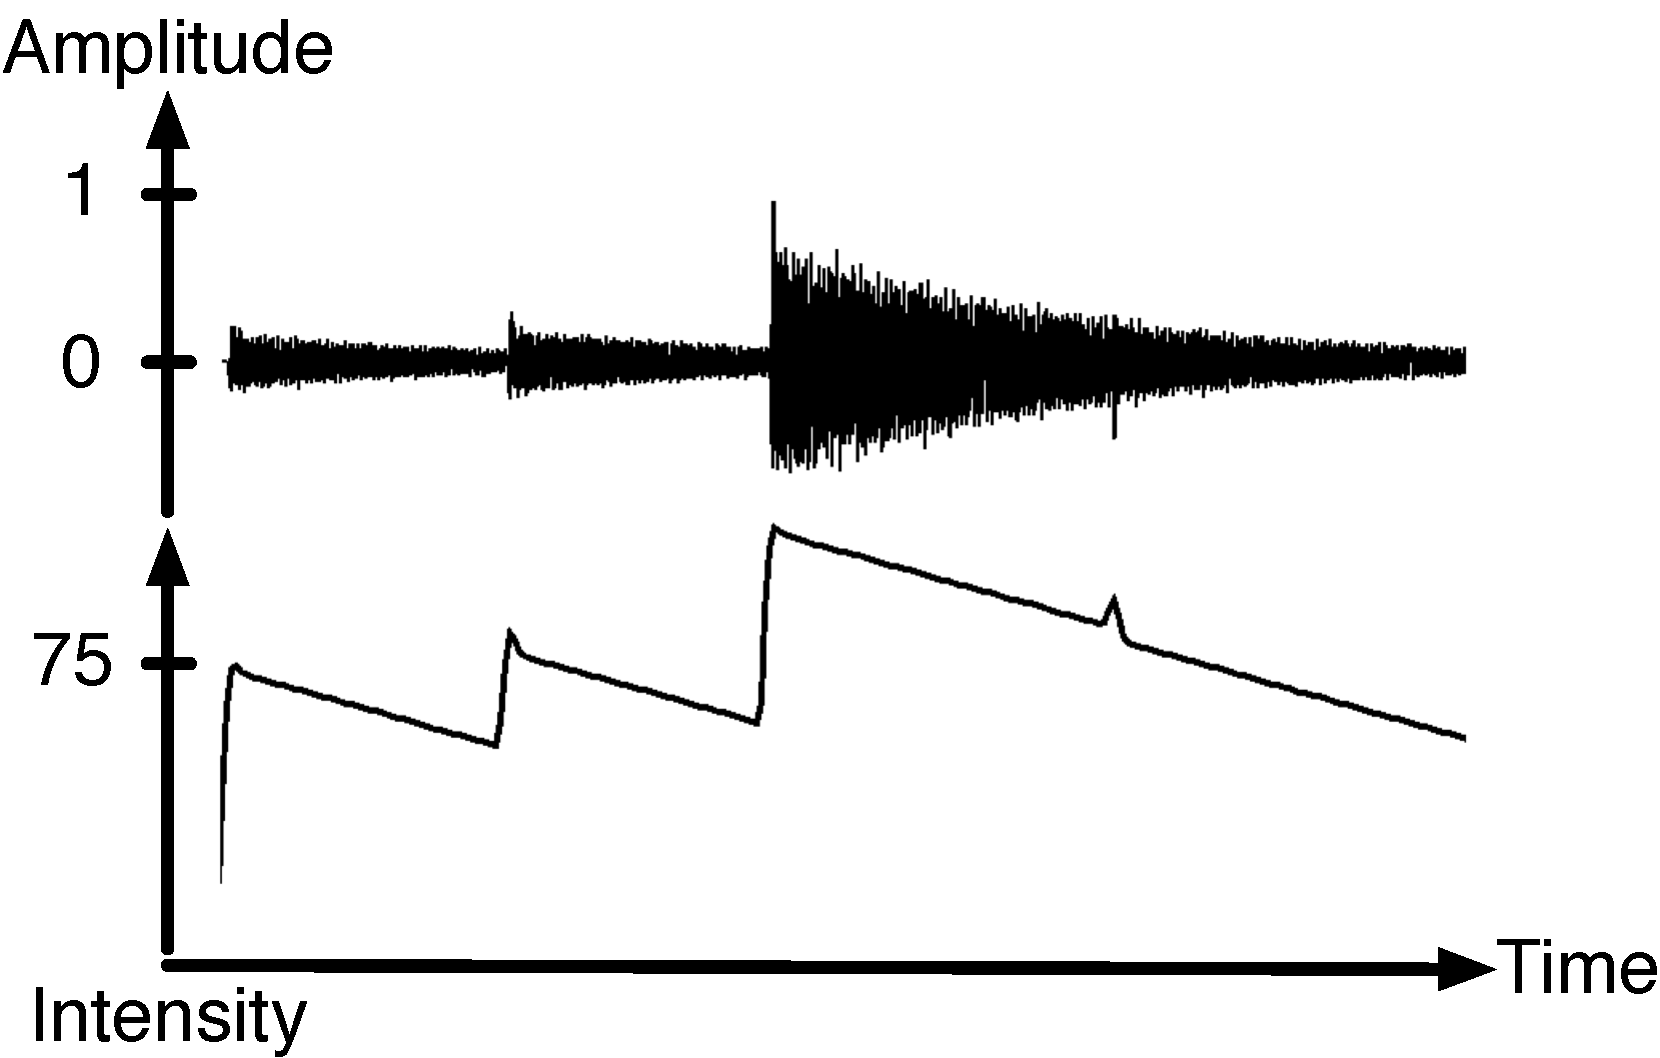
\includegraphics[width=0.4\linewidth]{Chapters/6/Pics/Pdf/soundComparison_waveAmplitude_1.pdf}}
		\hspace{6mm}
		\subfigure[]{\label{fig:soundComparison2}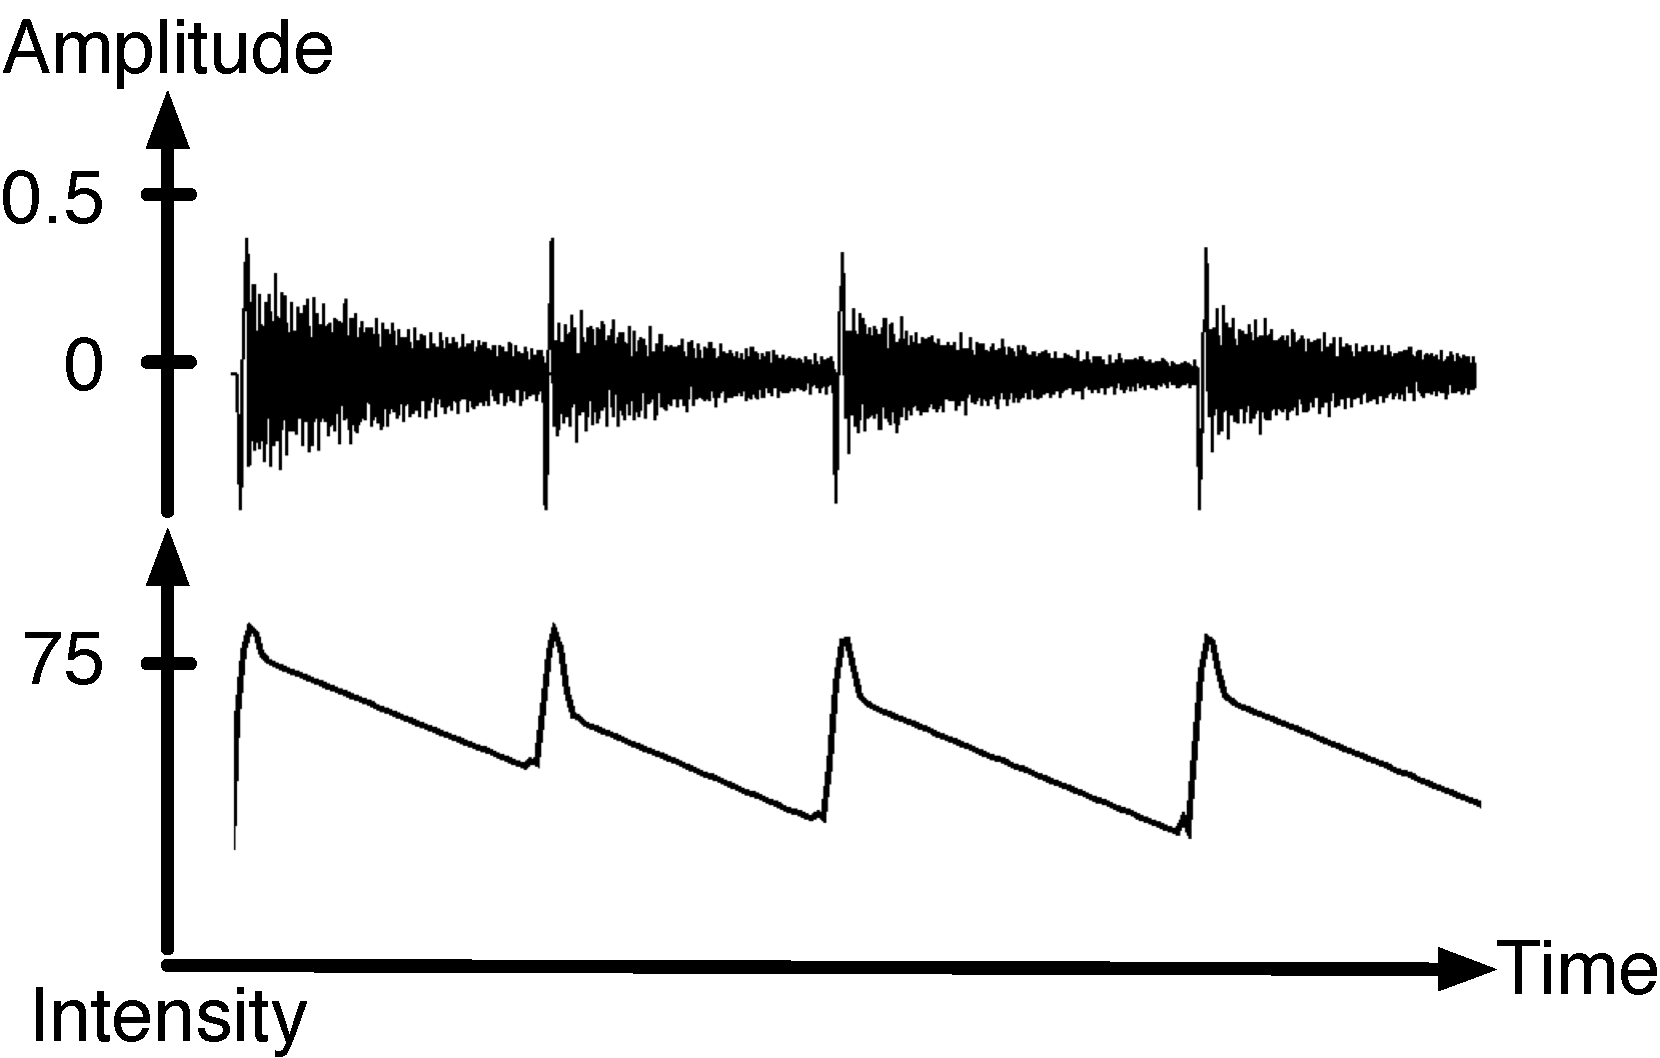
\includegraphics[width=0.4\linewidth]{Chapters/6/Pics/Pdf/soundComparison_waveAmplitude_2.pdf}}\\
		\subfigure[]{\label{fig:soundComparison3}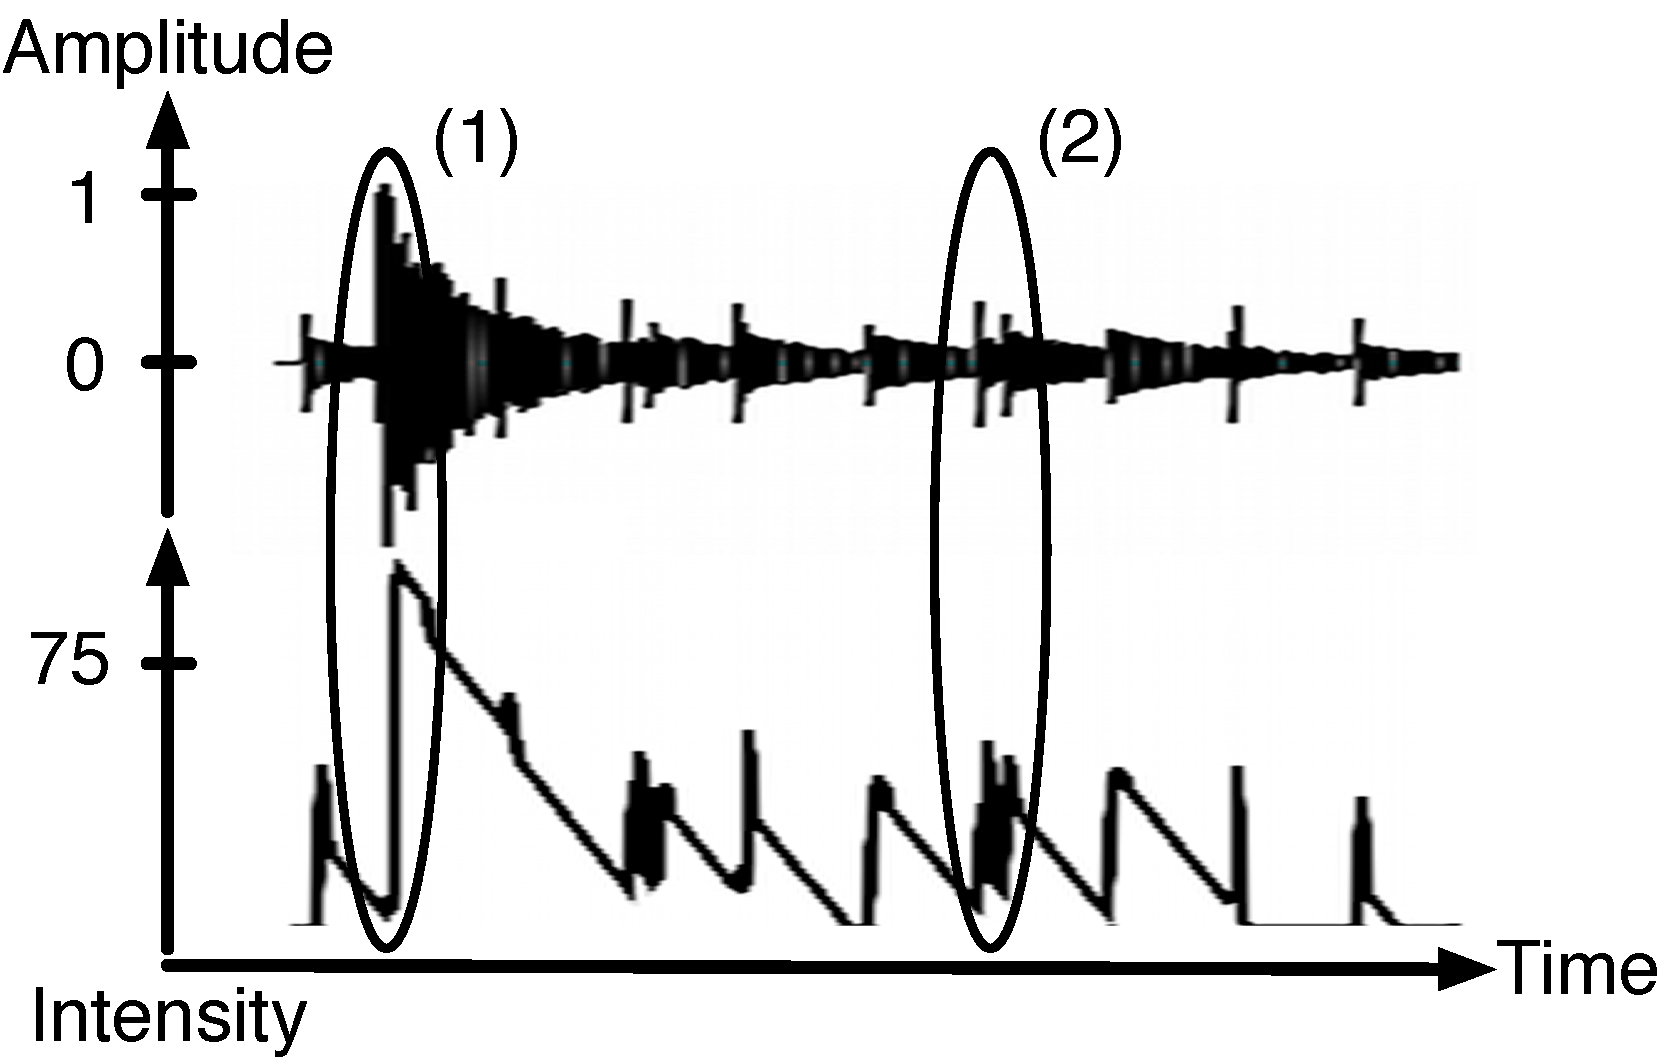
\includegraphics[width=0.4\linewidth]{Chapters/6/Pics/Pdf/soundComparison_waveAmplitude_3.pdf}}
	\end{center}
	\vspace{-0.5cm}
	\caption[Instrumental gesture simulation: artifacts and their influence on sound synthesis]{(a) A simulation artifact causes much larger sound waveform amplitude and sound intensity on the third beat, compared to (b) a stable simulation generating fairly constant amplitude and intensity for all beats. (c) Issues (1) and (2) discussed below: (1) artifact when two close beat impacts are glued together by the sound synthesis engine to form a huge sound, and issue (2) when two close beat impacts are finally heard.}
	\label{fig:soundComparison}
\end{figure}

Moreover, variations in the simulations of the two percussion grips can be found in the assembly of more complex gesture sequences. \emph{French} grip simulations work well, due to the large flexibility and smoothness of movement which lead to large amplitudes in the trajectories deployed by the human performer (cf. \myfigname \ref{fig:grips1}). The simulation framework is capable of following the original gesture trajectories and can articulate the sequence of gestures. For the \emph{German} grip though, due to the large motion-phase where the performer keeps the mallet relatively immobilized close to the membrane, the physics engine results are less satisfactory. This is mostly seen in sequences of gestures assembled from gesture units. The less successful simulation of \emph{German} grip can be due to two reasons.

The first reason is that our motion data does not take into account the fact that expert percussionists commonly use their fingers to help performing the strokes. This is true for both \emph{French} and \emph{German} grips, but the effect of this technique in the \emph{German} grip can be more important. The use of the \emph{German} grip involves generally a technique requiring more control from the wrist and fingers and less amplitude of the arms and forearms, in order to control the speed of the mallet as well as the duration of contact between the mallet and the timpani membrane.

The second reason reveals the fact that the mallets (and therefore the percussionists' arms) stay relatively immobile during a large portion of the gesture unit (cf. \myfigname \ref{fig:classifParameters}). It necessitates the simulation of fixed and more rigid postures that especially involve the tuning of the physical parameters with high stiffness values, thus potentially leading to instabilities in the numerical simulation. 
		
\myfigname \ref{fig:soundComparison3} shows the effect of this issue on the resulting sound. The virtual performer is given a task to perform a sequence of \emph{accent} strokes using captured data of the \emph{German} grip. From the resulting sounds, one can notice that at some moments, {\it (1)} the sound amplitude is largely superior to the average, and {\it (2)} the resulting beats are not regularly spaced, although no dynamics or tempo variation was present in the score. Issue {\it (1)} characterizes a larger stroke seen in the figure as an artifact from the sound synthesis generation, \emph{i.e.} the simulated gesture presents strokes that are very close temporally and spatially. The collision detection events, performed in a short lapse time, are then interpreted by the \emph{Modalys} system which "glues" them together as a single yet much stronger stroke. As for issue {\it (2)}, it can be explained by the limitations of both the capture database and the simulation framework, as discussed above. 


		\subsection{Motion Database and Gesture Edition}

Our framework depends highly on the motion clips initially recorded during the acquisition process of motion data. The motion database associated with edition processes are off-line components that are of particular importance when considering the composition of a gesture score. In this section we examine the assets and drawbacks of our system with respect to these components. We initially highlight the advantages of our framework in considering the simulation of percussion performances at the gestural level. We then discuss the completeness of the available motion capture database, as well as the editing method presented in this paper.


			\subsubsection{Advantages}

In this work, we adopted a sketching approach to the composition of gesture scores made of elementary gesture units. This constitutes an intuitive process where the user only needs to select and assemble a limited amount of canonical gesture units, one for representing each timpani playing mode. The gesture score can then be seen as copy-and-paste and concatenation processes of these gesture units to form a whole gesture score.\\

Although the presented model does not take into account the subtle articulation mechanisms occurring in real percussion performances, a simple articulation (interpolation) of gesture units is implicitly achieved by the internal physics simulation when the gesture score simulation switches from a gesture unit to another. Such a "sketching" approach has the advantage to be transparent to the user.\\

Another advantage of our framework in considering the composition at the gestural level is the preservation of the expressive features inherent to real percussion performances. As the composition process of gesture scores relies highly on real motion data, this insures that simulations will preserve the expressive components of the gesture units used in the gesture score. More interestingly, it allows consequently to preserve the style of the real performer in the simulated percussion performances. Specifically in this work, all the exercises presented in section \ref{sec:Music_Evaluation} have used motion data from one performer, such that these simulated exercises can be considered as supplementary exercises that we might have asked the percussionist to perform.\\

The presented motion capture database in section \ref{sec:Analysis_MoCapDatabase} focuses on a particular excerpt (grip, playing mode and beat location) among the multitude of percussion techniques used by timpani performers. Our system provides the interesting possibility of enriching this limited database by the editing and simulation of novel percussion performances. One can also consider our approach as a means of preventing the tedious and time-consuming task of capturing an exhaustive motion database containing all the possible combinations of playing techniques. %More specifically about the capture of music performances, such an approach prevents also from the worrying task of elaborating complex capturing settings to synchronize motion and sound data thanks to the physics-based framework. 
Finally, our framework provides an interactive tool that can be used in the exploration of the relationship between instrumental gestures and sound processes.


			\subsubsection{Limitations}

The motion capture database presented in section \ref{sec:Analysis_MoCapDatabase} focuses on specific set of timpani playing techniques, i.e. it provides gesture examples only for these playing techniques. As seen before, this fact limits the possible simulations to be performed with the proposed system.\\

Another limiting issue is the choice of the gesture units used during the editing step. As already discussed in the beginning of this chapter, such issue yields inevitably to the question of the existence of a best-suited gesture unit, compared to other examples of the same playing mode. If such "best" gesture unit exists, how can one identify it among the numerous replicates available in the motion database? Otherwise, does it make sense to average multiple gesture units so that a "mean" gesture unit can be used? We believe that using an average gesture might lead to the loss of some expressive features implicitly contained in the gesture signal. We therefore chose one specific gesture example within the sequence, without trying to find an optimization criteria for selecting this gesture unit.\\ %[Can you comment on the consequences of this arbitrary choice?]

A final issue to discuss related to the edition process is the concatenation of gesture units, which is the basis of the composition process. The gesture composition presented in this chapter is only based on a sketching process for composing gesture scores, therefore demonstrating the feasibility of the approach. It could be improved by considering higher-level planning processes responsible for the sequencing of gestures. In real percussion playing, high-level control mechanisms are indeed in charge of the articulation of playing modes, depending on many factors such as playing style, tempo variations as well as expressive nuances. Our concatenation model typically does not take such mechanisms into account.

%%%%%%%%%%%%%%%%%%%%%%%%%%%%%%%%%%%%%%%%%%%%%%%%%%%%%%%%%%%%%%%%%%%%%%%%%%%%%%%%%%%%%%%%%%%%%%%%%%%%%%%%%%%%%%%%%%%%


%%%%%%%%%%%%%%%%%%%%%%%%%%%%%%%%%%%%%%%%%%%%%%%%%%%%%%%%%%%%%%%%%%%%%%%%%%%%%%%%%%%%%%%%%%%%%%%%%%%%%%%%%%%%%%%%%%%%

	\section{Conclusion}
	\label{sec:Music_Conclusion}

This chapter presented a methodology for composing percussion exercises at the gestural level. This implies a sketching approach for assembling gesture units, leading to the synthesis of percussion exercises that were not initially recorded. The simulated exercises have explored both the composition of validation and extrapolation exercises, that were qualitatively evaluated by a percussion professor.

Validation exercises consist in assembling intra-gesture units, \emph{i.e.} the composition and simulation of gesture units of the same type. The evaluation of these exercises has underlined the accuracy and naturalness of the resulting simulations, both in terms of playing modes and impact locations. It was also pointed out some artifacts, such as gesture exaggeration and sound inaccuracies, that may be explained both in terms of the gesture simulation and sound models.

Extrapolation exercises have explored the articulation and simulation of various playing modes that were not recorded initially during the collection of motion capture data. The evaluation underlined the quality of the simulated articulation between these playing modes, as well as for the resulting sounds. Problems in these simulations were mainly cause by the lack of completeness of the motion capture database.

%This accelerando-decelerando exercise explored the articulation of \emph{legato} strokes under a tempo variation. Here again one can notice the quality of the simulated accelerando-decelerando from simulation effects such as a crescendo effect on the resulting sound. Issues related to the motion amplitude have been interpreted as a consequence of the \emph{limited} playing expertise of the virtual percussionist.

%%%%%%%%%%%%%%%%%%%%%%%%%%%%%%%%%%%%%%%%%%%%%%%%%%%%%%%%%%%%%%%%%%%%%%%%%%%%%%%%%%%%%%%%%%%%%%%%%%%%%%%%%%%%%%%%%%%%
